%Este trabalho está licenciado sob a Licença Atribuição-CompartilhaIgual 4.0 Internacional Creative Commons. Para visualizar uma cópia desta licença, visite http://creativecommons.org/licenses/by-sa/4.0/deed.pt_BR ou mande uma carta para Creative Commons, PO Box 1866, Mountain View, CA 94042, USA.

\chapter{Métodos para Sistemas Lineares}\label{cap_sislin}

Neste capítulo, discutimos sobre métodos diretos para a resolução de sistemas lineares de $n$-equações com $n$-incógnitas. Isto é, sistemas que podem ser escritos na seguinte \hl{\emph{forma algébrica}}
\begin{subequations}
  \begin{align}
    &a_{11}x_1 + a_{12}x_2 + \cdots + a_{1n}x_n = b_1\\
    &a_{21}x_1 + a_{22}x_2 + \cdots + a_{2n}x_n = b_2\\
    &\quad\quad\vdots \\
    &a_{n1}x_1 + a_{n2}x_2 + \cdots + a_{nn}x_n = b_n.
  \end{align}
\end{subequations}
Equivalentemente, o sistema pode ser escrito na \hl{\emph{forma matricial}}
\begin{equation}\hleq
  A\pmb{x} = \pmb{b}
\end{equation}
onde, $A = [a_{i,j}]_{i,j=1}^{n,n}$ é a \hl{\emph{matriz dos coeficientes}}
\begin{equation}
  A =
  \begin{bmatrix}
    a_{1,1} & a_{1,2} & \ldots & a_{1,n}\\
    a_{2,1} & a_{2,2} & \ldots & a_{2,n}\\
    \vdots & \vdots & \ddots & \vdots\\
    a_{n,1} & a_{n,2} & \ldots & a_{n,n}\\
  \end{bmatrix},
\end{equation}
o \hl{\emph{vetor das incógnitas}} $\pmb{x} = (x_i)_{i=1}^n$ é
\begin{equation}
  \pmb{x} =
  \begin{bmatrix}
    x_1\\
    x_2\\
    \vdots\\
    x_n
  \end{bmatrix}
\end{equation}
e o \hl{\emph{vetor dos termos constantes}} $\pmb{b} = (b_i)_{i=1}^n$ é
\begin{equation}
  \pmb{b} =
  \begin{bmatrix}
    b_1\\
    b_2\\
    \vdots\\
    b_n
  \end{bmatrix}
\end{equation}

\section{Método da Decomposição LU}\label{cap_sislin_sec_lu}

O Método da Decomposição LU é uma forma eficiente de se resolver sistemas lineares de pequeno porte. \hl{Dado um sistema $A\pmb{x} = \pmb{b}$, a ideia é decompor a matriz $A$ como o produto de uma \emph{matriz triangular inferior} $L$ (do inglês, \textit{lower triangular matrix}) com uma \emph{matriz triangular superior} $U$ (do inglês, \textit{upper triangular matrix})}, i.e.
\begin{equation}
  \hleq A = LU.
\end{equation}
Com isso, o sistema pode ser reescrito na forma
\begin{gather}
  A\pmb{x} = \pmb{b}\\
  (LU)\pmb{x} = \pmb{b}\\
  L(U\pmb{x}) = \pmb{b}.
\end{gather}
Denotando,
\begin{equation}
  U\pmb{x} =: \emph{y}
\end{equation}
podemos resolver o seguinte sistema triangular
\begin{equation}
  L\pmb{y} = \pmb{b}.
\end{equation}
Tendo resolvido este sistema, a solução do sistema $A\pmb{x} = \pmb{b}$ pode, então, ser computada como a solução do sistema triangular
\begin{equation}
  U\pmb{x} = \pmb{y}.
\end{equation}
Ou seja, \hl{a decomposição LU nos permite resolver uma sistema pela resolução de dois sistemas triangulares}.

\subsection{Sistemas Triangulares}

Antes de estudarmos como podemos computar a decomposição LU de uma matriz, vamos discutir sobre a resolução de sistemas triangulares.

\subsubsection{Sistema Triangular Inferior}

\hl{Um \emph{sistema linear triangular inferior}} tem a forma algébrica
\begin{equation}
  \begin{matrix}
    a_{1,1}x_1 &&&&&= b_1\\
    a_{2,1}x_1 &+ a_{2,2}x_2 &&&&= b_2\\
    \vdots &&&&& \vdots\\
    a_{n-1,1}x_1 &+ a_{n-1,2}x_2 &+ \cdots &+ a_{n-1,n-1}x_{n-1} &&= b_{n-1}\\
    a_{n,1}x_1 &+ a_{n,2}x_2 &+ \cdots &+ a_{n,n-1}x_{n-1} &+ a_{n,n}x_n &= b_n
  \end{matrix}
\end{equation}
\hl{Pode ser diretamente resolvido de cima para baixo}, i.e.
\begin{align}
  x_1 &= \frac{b_1}{a_{1,1}}\\
  x_2 &= \frac{b_{2} - a_{2,1}x_1}{a_{2,2}}\\
      &\vdots\\
  x_n &= \frac{b_n - a_{n,1}x_1 - a_{n,2}x_2 - \ldots - a_{n,n-1}x_{n-1}}{a_{n,n}}
\end{align}

\begin{ex}
  Vamos resolver o sistema triangular inferior
  \begin{equation}
    \begin{matrix}
      x_1 &&&= 2\\
      -3x_1 &+ 2x_2 &&= -8\\
      -x_1 &+ x_2 &- x_3 &= 0
    \end{matrix}
  \end{equation}
  Na primeira equação, temos
  \begin{equation}
    x_1 = 2
  \end{equation}
  Então, da segunda equação do sistema
  \begin{gather}
    -3x_1 + 2x_2 = -8\\
    x_2 = \frac{-8 + 3x_1}{2}\\
    x_2 = \frac{-8 + 3\cdot 2}{2}\\
    x_2 = -1
  \end{gather}
  E, por fim, da última equação
  \begin{gather}
    -x_1 + x_2 - x_3 = 0\\
    x_3 = \frac{x_1 - x_2}{-1}\\
    x_3 = \frac{2 - (-1)}{-1}\\
    x_3 = 3
  \end{gather}
  Concluímos que a solução do sistema é $\pmb{x} = (2, -1, 3)$.

\begin{lstlisting}[caption=solSisTriaInf.py, label=cap_sislin_sec_lu:cod:solSisTriaInf]
import numpy as np

def solSisTriaInf(A, b):
  n = b.size
  x = np.zeros_like(b)
  for i in range(n):
    x[i] = b[i]
    for j in range(i):
      x[i] -= A[i,j]*x[j]
    x[i] /= A[i,i]
  return x    

# mat coefficientes
A = np.array([[1., 0., 0.],
              [-3., 2., 0.],
              [-1., 1., -1.]])

# vet termos constantes
b = np.array([2., -8., 0.])

# resol sis lin
x = solSisTriaInf(A, b)
print(x)
\end{lstlisting}

\end{ex}

\begin{obs}\normalfont{(\hl{Número de operações em ponto flutuante}.)}
  A computação da solução de um sistema $n\times n$ triangular inferior requer $O(n^2)$ operações em ponto flutuante (multiplicações/divisões e adições/subtrações).
\end{obs}

\subsubsection{Sistema Triangular Superior}

\hl{Um \emph{sistema linear triangular superior}} tem a forma algébrica
\begin{equation}
  \begin{matrix}
    a_{1,1}x_1 &+ a_{1,2}x_2 &+ \cdots &+ a_{1,n}x_n &= b_1\\
              &a_{2,2}x_2  &+ \cdots &+ a_{2,n}x_{n} &= b_2\\
              &&& \vdots  &\vdots \\
              &&& a_{n,n}x_n &= b_n
  \end{matrix}
\end{equation}
\hl{Pode ser diretamente resolvido de baixo para cima}, i.e.
\begin{align}
  x_n &= \frac{b_n}{a_{n,n}}\\
  x_{n-1} &= \frac{b_{n-1} - a_{n-1,n}x_n}{a_{n-1,n-1}}\\
      &\vdots\\
  x_n &= \frac{b_1 - a_{1,1}x_1 - a_{1,2}x_2 - \ldots - a_{1,n-1}x_{n-1}}{a_{1,1}}
\end{align}

\begin{ex}
  Vamos resolver o sistema triangular superior
  \begin{equation}
    \begin{matrix}
      2x_1 &- x_2 &+ 2x_3 &= 7\\
      & 2x_2 &- x_3 &= -3\\
      &&3x_3 &= 3
    \end{matrix}
  \end{equation}
  Da última equação, temos
  \begin{gather}
    x_3 = \frac{3}{3}\\
    x_3 = 1
  \end{gather}
  Então, da segunda equação do sistema, obtemos
  \begin{gather}
    2x_2 - x_3 = -3\\
    x_2 = \frac{x_3 - 3}{2}\\
    x_2 = \frac{1 - 3}{2}\\
    x_2 = -1
  \end{gather}
  Por fim, da primeira equação
  \begin{gather}
    2x_1 - x_2 + 2x_3 = 7\\
    x_1 = \frac{7 + x_2 - 2x_3}{2}\\
    x_1 = \frac{7 - 1 - 2}{2}\\
    x_1 = 2
  \end{gather}
  Concluímos que a solução do sistema é $\pmb{x} = (2, -1, 1)$.

\begin{lstlisting}[caption=solSisTriaSup.py, label=cap_sislin_sec_lu:cod:solSisTriaSup]
import numpy as np

def solSisTriaSup(A, b):
  n = b.size
  x = np.zeros_like(b)
  for i in range(n-1,-1,-1):
    x[i] = b[i]
    for j in range(n-1,i,-1):
      x[i] -= A[i,j]*x[j]
    x[i] /= A[i,i]
  return x
    

# mat coefficientes
A = np.array([[2., -1., 2.],
              [0., 2., -1.],
              [0., 0., 3.]])

# vet termos constantes
b = np.array([7., -3., 3.])

# sol sis lin
x = solSisTriaSup(A, b)
print(x)
\end{lstlisting}

\end{ex}

\begin{obs}\normalfont{(\hl{Número de operações em ponto flutuante}.)}
  A computação da solução um sistema $n\times n$ triangular superior requer $O(n^2)$ operações em ponto flutuante (multiplicações/divisões e adições/subtrações).
\end{obs}

\subsection{Decomposição LU}

\hl{O procedimento da decomposição LU é equivalente ao método de eliminação gaussiana}. Consideramos uma matriz $A = [a_{ij}]_{i,j=1}^{n,n}$, com $a_{1,1}\neq 0$, e começamos denotando esta matriz por $U^{(0)} = [u_{i,j}^{(0)}]_{i,j=1}^{n,n} = A$ e tomando $L^{(0)} = I_{n\times n}$. A eliminação abaixo do pivô $u_{1,1}^{(0)}$, pode ser computada com as seguintes operações equivalentes por linha
\begin{equation}
  U^{(0)} = \begin{bmatrix}
    u_{1,1}^{(0)} & u_{1,2}^{(0)} & u_{1,3}^{(0)} & \ldots & u_{1,n}^{(0)} \\
    u_{2,1}^{(0)} & u_{2,2}^{(0)} & u_{2,3}^{(0)} & \ldots & u_{2,n}^{(0)} \\
    u_{3,1}^{(0)} & u_{3,2}^{(0)} & u_{3,3}^{(0)} & \ldots & u_{3,n}^{(0)} \\
    \vdots & \vdots & \vdots & \ldots & \vdots \\
    u_{n,1}^{(0)} & u_{n,2}^{(0)} & a_{n,3}^{(0)} & \ldots & u_{n,n}^{(0)}
  \end{bmatrix}
  \begin{array}{l}
    U_1^{(1)} \leftarrow U_1^{(0)}\\
    U_2^{(1)} \leftarrow U_2^{(0)} - l_{2,1}^{(1)}U_1^{(0)}\\
    U_3^{(1)} \leftarrow U_3^{(0)} - l_{3,1}^{(1)}U_1^{(0)}\\
    \vdots\\
    U_n^{(1)} \leftarrow U_n^{(0)} - l_{n,1}^{(1)}U_1^{(0)}
  \end{array}
\end{equation}
onde, $l_{i,1}^{(1)}=u_{i,1}^{(0)}/u_{1,1}^{(0)}$, $i=2, 3, \dotsc, n$.

Destas computações, obtemos uma nova matriz da forma
\begin{equation}
  U^{(1)} = \begin{bmatrix}
    u_{1,1}^{(1)} & u_{1,2}^{(1)} & u_{1,3}^{(1)} & \ldots & u_{1,n}^{(1)} \\
    0 & u_{2,2}^{(1)} & u_{2,3}^{(1)} & \ldots & u_{2,n}^{(1)} \\
    0 & u_{3,2}^{(1)} & u_{3,3}^{(1)} & \ldots & u_{3,n}^{(1)} \\
    \vdots & \vdots & \vdots & \ldots & \vdots \\
    0 & u_{n,2}^{(1)} & u_{n,3}^{(1)} & \ldots & u_{n,n}^{(1)}
  \end{bmatrix}  
\end{equation}
E, denotando
\begin{equation}
  L^{(1)} =
  \begin{bmatrix}
    1 & 0 & 0 & \ldots & 0\\
    l_{2,1}^{(1)} & 1 & 0 & \ldots & 0\\
    l_{3,1}^{(1)} & 0 & 1 & \ldots & 0\\
    \vdots & \vdots & \vdots & \ldots & \vdots\\
    l_{n,1}^{(1)} & 0 & 0 & \ldots & 1
  \end{bmatrix}
\end{equation}
temos
\begin{equation}
  A = L^{(1)}U^{(1)}.
\end{equation}
No caso de $u^{(1)}_{2,2}\neq 0$, podemos continuar com o procedimento de eliminação gaussiana com as seguintes operações equivalentes por linha
\begin{equation}
  U^{(1)} = \begin{bmatrix}
    u_{1,1}^{(1)} & u_{1,2}^{(1)} & u_{1,3}^{(1)} & \ldots & u_{1,n}^{(1)} \\
    0 & u_{2,2}^{(1)} & u_{2,3}^{(1)} & \ldots & u_{2,n}^{(1)} \\
    0 & u_{3,2}^{(1)} & u_{3,3}^{(1)} & \ldots & u_{3,n}^{(1)} \\
    \vdots & \vdots & \vdots & \ldots & \vdots \\
    0 & u_{n,2}^{(1)} & u_{n,3}^{(1)} & \ldots & u_{n,n}^{(1)}
  \end{bmatrix}  
  \begin{array}{l}
    U_1^{(2)}\leftarrow U_1^{(1)}\\
    U_2^{(2)}\leftarrow U_2^{(1)}\\
    U_3^{(2)} \leftarrow U_3^{(1)} - l_{3,2}^{(2)}U_2^{(1)}\\
    \vdots\\
    U_n^{(2)} \leftarrow U_n^{(1)} - l_{n,2}^{(2)}U_2^{(1)}\\
  \end{array}
\end{equation}
onde, $l_{i,2}^{(2)} = u_{i,2}^{(1)}/u_{2,2}^{(1)}$, $i=3, 4, \ldots, n$. Isto nos fornece
o que nos fornece
\begin{equation}
  U^{(2)} = \begin{bmatrix}
    u_{1,1}^{(2)} & u_{1,2}^{(2)} & u_{1,3}^{(2)} & \ldots & u_{1,n}^{(2)} \\
    0 & u_{2,2}^{(2)} & u_{2,3}^{(2)} & \ldots & u_{2,n}^{(2)} \\
    0 & 0 & u_{3,3}^{(2)} & \ldots & u_{3,n}^{(2)} \\
    \vdots & \vdots & \vdots & \ldots & \vdots \\
    0 & 0 & u_{n,3}^{(2)} & \ldots & u_{n,n}^{(2)}
  \end{bmatrix}.
\end{equation}
Além disso, denotando
\begin{equation}
  L^{(2)} =
  \begin{bmatrix}
    1 & 0 & 0 & \ldots & 0\\
    l_{2,1}^{(1)} & 1 & 0 & \ldots & 0\\
    l_{3,1}^{(1)} & l_{3,2}^{(2)} & 1 & \ldots & 0\\
    \vdots & \vdots & \vdots & \ldots & \vdots\\
    l_{n,1}^{(1)} & l_{n,2}^{(2)} & 0 & \ldots & 1
  \end{bmatrix}
\end{equation}
temos
\begin{equation}
  A = L^{(2)}U^{(2)}.
\end{equation}
Continuando com este procedimento, ao final de $n-1$ passos teremos obtido a decomposição
\begin{equation}
  A = LU,
\end{equation}
onde $L$ é a matriz triangular inferior
\begin{equation}
  L = L^{(n-1)} =   \begin{bmatrix}
    1 & 0 & 0 & \ldots & 0\\
    l_{2,1}^{(1)} & 1 & 0 & \ldots & 0\\
    l_{3,1}^{(1)} & l_{3,2}^{(2)} & 1 & \ldots & 0\\
    \vdots & \vdots & \vdots & \ldots & \vdots\\
    l_{n,1}^{(1)} & l_{n,2}^{(2)} & l_{n,3}^{(3)} & \ldots & 1
  \end{bmatrix}
\end{equation}
e $U$ é a matriz triangular superior
\begin{equation}
  U = U^{(n-1)} = \begin{bmatrix}
    u_{1,1}^{(0)} & u_{1,2}^{(0)} & u_{1,3}^{(0)} & \ldots & u_{1,n}^{(0)} \\
    0 & u_{2,2}^{(1)} & u_{2,3}^{(1)} & \ldots & u_{2,n}^{(1)} \\
    0 & 0 & u_{3,3}^{(2)} & \ldots & u_{3,n}^{(2)} \\
    \vdots & \vdots & \vdots & \ldots & \vdots \\
    0 & 0 & 0 & \ldots & u_{n,n}^{(n-1)}
  \end{bmatrix}.
\end{equation}

\begin{ex}\label{ex:lu}
  Consideramos a seguinte matriz
  \begin{equation}
    A =
    \begin{bmatrix}
      -1 & 2 & -2\\
      3 & -4 & 1\\
      1 & -5 & 3
    \end{bmatrix}.
  \end{equation}
  Para obtermos sua decomposição $LU$ começamos com
  \begin{align}
    L^{(0)} &:=
    \begin{bmatrix}
      1 & 0 & 0\\
      0 & 1 & 0\\
      0 & 0 & 1
    \end{bmatrix},\\
    U^{(0)} &:=
    \begin{bmatrix}
      -1 & 2 & -2\\
      3 & -4 & 1\\
      1 & -5 & 3
    \end{bmatrix}.
  \end{align}
  Então, observando que a eliminação abaixo do pivô $u_{1,1}=-1$ pode ser feita com as seguintes operações equivalentes por linha
  \begin{equation}
    U^{(0)} =
    \begin{bmatrix}
      -1 & 2 & -2\\
      3 & -4 & 1\\
      1 & -5 & 3
    \end{bmatrix}
    \begin{array}{l}
      U_1^{(1)}\leftarrow U_1^{(0)}\\
      U_2^{1}\leftarrow U_2^{(0)} - \frac{3}{-1}U_1^{(0)}\\
      U_3^{1}\leftarrow U_3^{(0)} - \frac{1}{-1}U_1^{(0)}
    \end{array},
  \end{equation}
  temos
  \begin{align}
    L^{(1)} &:=
    \begin{bmatrix}
      1 & 0 & 0\\
      -3 & 1 & 0\\
      -1 & 0 & 1
    \end{bmatrix},\\
    U^{(1)} &:=
    \begin{bmatrix}
      -1 & 2 & -2\\
      0 & 2 & -5\\
      0 & -3 & 1
    \end{bmatrix}.
  \end{align}
  Agora, para eliminarmos abaixo do pivô $u_{2,2}=2$, usamos as operações
  \begin{equation}
    U^{(1)} :=
    \begin{bmatrix}
      -1 & 2 & -2\\
      0 & 2 & -5\\
      0 & -3 & 1
    \end{bmatrix}
    \begin{array}[]l
      U_1^{(2)}\leftarrow U_1^{(1)} \\
      U_2^{(2)}\leftarrow U_2^{(1)} \\
      U_3^{(2)}\leftarrow U_3^{(1)} - \frac{-3}{2}U_2^{(1)}
    \end{array},
  \end{equation}
  donde
  \begin{align}
    L^{(2)} =
    \begin{bmatrix}
      1 & 0 & 0\\
      -3 & 1 & 0\\
      -1 & -1.5 & 1
    \end{bmatrix},\\
    U^{(1)} =
    \begin{bmatrix}
      -1 & 2 & -2\\
      0 & 2 & -5\\
      0 & 0 & -6.5
    \end{bmatrix}.
  \end{align}
Isso completa a decomposição, sendo $L := L^{(3)}$ e $U := U^{(3)}$.

\begin{lstlisting}[caption=lu.py, label='cap_sislin_sec_lu:cod:lu']
import numpy as np

def lu(A):
  # num. de linhas
  n = A.shape[0]

  # inicialização
  U = A.copy()
  L = np.eye(n)

  # decomposição
  for i in range(n-1):
    for j in range(i+1,n):
        L[j,i] = U[j,i]/U[i,i]
        U[j,i:] -= L[j,i]*U[i,i:]

  return L, U

# matriz
A = np.array([[-1., 2., -2.],
              [3., -4., 1.],
              [1., -5., 3.]])

L, U = lu(A)
\end{lstlisting}

\end{ex}

\begin{obs}\normalfont{(\hl{Número de operações em ponto flutuante}.)}
  A decomposição LU de um sistema $n\times n$ requer $O(n^3)$ operações em ponto flutuante (multiplicações/divisões e adições/subtrações).
\end{obs}


\subsection{Resolução do Sistema com Decomposição LU}

Consideramos o sistema linear
\begin{equation}
  A\pmb{x} = \pmb{b}.
\end{equation}

Para resolvê-lo com o \hl{Método LU}, fazemos
\begin{enumerate}[1.]
\item \hl{Computamos a decomposição LU}
  \begin{equation}\hleq
    A = LU.
  \end{equation}
\item \hl{Resolvemos o sistema triangular inferior}
  \begin{equation}\hleq
    L\pmb{y} = \pmb{b}.
  \end{equation}
\item \hl{Resolvemos o sistema triangular superior}
  \begin{equation}\hleq
    U\pmb{x} = \pmb{y}.
  \end{equation}
\end{enumerate}

\begin{ex}\label{ex:lu}
  Vamos resolver o seguinte sistema linear
  \begin{equation}
    \begin{aligned}
      -x_1 + 2x_2 - 2x_3 &= 6\\
      3x_1 - 4x_2 + x_3 &= -11\\
      x_1 - 5x_2 + 3x_3 &= -10.
    \end{aligned}
\end{equation}
  No exemplo anterior (Exemplo \ref{ex:lu}), vimos que a matriz de coeficientes $A$ deste sistema admite a seguinte decomposição LU
  \begin{equation}
    \underbrace{\begin{bmatrix}
      -1 & 2 & -2\\
      3 & -4 & 1\\
      1 & -5 & 3
    \end{bmatrix}}_{A} =
  \underbrace{\begin{bmatrix}
      1 & 0 & 0\\
      -3 & 1 & 0\\
      -1 & -1.5 & 1
    \end{bmatrix}}_{L}
  \underbrace{\begin{bmatrix}
      -1 & 2 & -2\\
      0 & 2 & -5\\
      0 & 0 & -6.5
    \end{bmatrix}}_{U}
  \end{equation}
  Daí, iniciamos resolvendo o seguinte sistema triangular inferior $Ly = b$, i.e.
  \begin{align}
    &\hleq{y_1 = 6} \\
    &-3y_1 + y_2 = -11 \\
    &\qquad\Rightarrow \hleq{y_2 = 7}\\
    &-y_1 - 1.5y_2 + y_3 = -10 \\
    &\qquad\Rightarrow \hleq{y_3 = 6.5}.
  \end{align}
  Por fim, computamos a solução $x$ resolvendo o sistema triangular superior $Ux=y$, i.e.
  \begin{align}
    &-6.5x_3 = 6.5 \\
    &\qquad \Rightarrow \hleq{x_3 = -1},\\
    &2x_2 - 5x_3 = 7 \\
    &\qquad \Rightarrow \hleq{x_2 = 1}\\
    &-x_1 + 2x_2 - 2x_3 = 6 \\
    &\qquad \Rightarrow \hleq{x_1 = -2}.
  \end{align}

\begin{lstlisting}
import numpy as np

# mat coefs
A = np.array([[-1., 2., -2.],
              [3., -4., 1.],
              [1., -5., 3.]])
# vet termos const
b = np.array([6., -11., -10.])

# 1. LU
L, U = lu(A)

# 2. Ly = b
y = solSisTriaInf(L, b)

# 3. Ux = y
x = solSisTriaSup(U, y)
\end{lstlisting}

\end{ex}

\subsection{Fatoração LU com Pivotamento Parcial}

O algoritmo estudando acima não é aplicável no caso de o pivô ser nulo, o que pode ser corrigido através de permutações de linhas. \hl{Na fatoração LU com pivotamento parcial fazemos permutações de linha na matriz de forma que o pivô seja sempre aquele de maior valor em módulo}. Por exemplo, suponha que o elemento $a_{3,1}$ seja o maior valor em módulo na primeira coluna da matriz $A = U^{(0)}$ com
\begin{equation}
  U^{(0)} = \begin{bmatrix}
    u_{1,1}^{(0)} & u_{1,2}^{(0)} & u_{1,3}^{(0)} & \ldots & u_{1,n}^{(0)} \\
    u_{2,1}^{(0)} & u_{2,2}^{(0)} & u_{2,3}^{(0)} & \ldots & u_{2,n}^{(0)} \\
    \pmb{u_{3,1}^{(0)}} & u_{3,2}^{(0)} & u_{3,3}^{(0)} & \ldots & u_{3,n}^{(0)} \\
    \vdots & \vdots & \vdots & \ldots & \vdots \\
    u_{n,1}^{(0)} & u_{n,2}^{(0)} & a_{n,3}^{(0)} & \ldots & u_{n,n}^{(0)}
  \end{bmatrix}.
\end{equation}
Neste caso, o procedimento de eliminação na primeira coluna deve usar $u_{3,1}^{(0)}$ como pivô, o que requer a permutação entre as linhas $1$ e $3$ ($U_1^{(0)} \leftrightarrow U_3^{(0)}$). Isto pode ser feito utilizando-se da seguinte \emph{matriz de permutação}
\begin{equation}
  P =
  \begin{bmatrix}
    0 & 0 & 1 & \ldots & 0\\
    0 & 1 & 0 & \ldots & 0\\
    1 & 0 & 0 & \ldots & 0\\
    \vdots & \vdots & \vdots & \ldots & \vdots\\
    0 & 0 & 0 & \ldots & 1
  \end{bmatrix}.
\end{equation}
Com essa, iniciamos o procedimento de decomposição LU com $PA = L^{(0)}U^{(0)}$, onde $L^{(0)} = I_{n\times n}$ e $U^{(0)} = PA$. Caso sejam necessárias outras mudanças de linhas no decorrer do procedimento de decomposição, a matriz de permutação $P$ deve ser atualizada apropriadamente.

\begin{ex}\label{cap_sislin_sec_lu:ex:lup}
  Vamos fazer a decomposição LU com pivotamento parcial da seguinte matriz
  \begin{equation}
    A = \begin{bmatrix}
      -1 & 2 & -2\\
      3 & -4 & 1\\
      1 & -5 & 3
    \end{bmatrix}
  \end{equation}
  Começamos, tomando
  \begin{align}
    P^{(0)} =
    \begin{bmatrix}
      1 & 0 & 0\\
      0 & 1 & 0\\
      0 & 0 & 1
    \end{bmatrix},\\
    L^{(0)} =
    \begin{bmatrix}
      1 & 0 & 0\\
      0 & 1 & 0\\
      0 & 0 & 1      
    \end{bmatrix},\\
    U^{(0)} = 
    \begin{bmatrix}
      -1 & 2 & -2\\
      3 & -4 & 1\\
      1 & -5 & 3
    \end{bmatrix}
  \end{align}
  O candidato a pivô é o elemento $u^{(0)}_{2,1}$. Então, fazemos as permutações de linhas
  \begin{align}
    P_1^{((0)} &\leftrightarrow P_2^{(0)},\\
    U_1^{(0)} &\leftrightarrow U_2^{(0)}
  \end{align}
  e, na sequência, as operações elementares por linhas
  \begin{equation}
    U_{2:3}^{(1)}\leftarrow U_{2:3}^{(0)}-m^{(0)}_{2:3,1}U_1^{(0)},
  \end{equation}
  donde obtemos
  \begin{align}
    P^{(1)} &=
    \begin{bmatrix}
      0 & 1 & 0\\
      1 & 0 & 0\\
      0 & 0 & 1
    \end{bmatrix},\\
    L^{(1)} &=
    \begin{bmatrix}
      1 & 0 & 0\\
      -0,\overline{3} & 1 & 0\\
      0,\overline{3} & 0 & 1      
    \end{bmatrix},\\
    U^{(1)} &= 
    \begin{bmatrix}
      3 & -4 & 1\\
      0 & 0,\overline{6} & -1,\overline{6}\\
      0 & -3,\overline{6} & 2,\overline{6}
    \end{bmatrix}
  \end{align}
  Agora, o candidato a pivô é o elemento $u^{(1)}_{3,2}$. Assim, fazemos as permutações de linhas
  \begin{align}
    P^{(1)}_2 &\leftrightarrow P^{(1)}_3, \\
    U^{(1)}_2 &\leftrightarrow U^{(1)}_3
  \end{align}
  e análogo para os elementos da coluna 1 de $L$. Então, fazemos a operação elementar por linha
  \begin{equation}
    U^{(2)}_3 \leftarrow U^{(1)}_3 - m^{(1)}_{3,2}U^{(1)}_2
  \end{equation}
. Com isso, obtemos
  \begin{align}
    P^{(2)} &=
    \begin{bmatrix}
      0 & 1 & 0\\
      0 & 0 & 1\\
      1 & 0 & 0
    \end{bmatrix},\\
    L^{(2)} &=
    \begin{bmatrix}
      1 & 0 & 0\\
      0,\overline{3} & 1 & 0\\
      -0,\overline{3} & -0,\overline{18} & 1      
    \end{bmatrix},\\
    U^{(2)} &= 
    \begin{bmatrix}
      3 & -4 & 1\\
      0 & -3,\overline{6} & 2,\overline{6}\\
      0 & 0 & -1,\overline{18}
    \end{bmatrix}
  \end{align}
  Por fim, temos obtido a decomposição LU de $A$ na forma
  \begin{equation}
    PA = LU,
  \end{equation}
  com $P=P^{(2)}$, $L=L^{(2)}$ e $U=U^{(2)}$.

\begin{lstlisting}[caption=lup.py, label=cap_sislin_sec_lu:cod:lup]
import numpy as np

def lup(A):
  # num. de linhas
  n = A.shape[0]

  # inicialização
  U = A.copy()
  L = np.eye(n)
  P = np.eye(n)

  # decomposição
  for i in range(n-1):
    # permutação de linhas
    p = i + np.argmax(np.fabs(U[i:,i]))
    P[[i,p]] = P[[p,i]]
    U[[i,p]] = U[[p,i]]
    L[[i,p],:i] = L[[p,i],:i]
    # eliminação gaussiana
    for j in range(i+1,n):
      L[j,i] = U[j,i]/U[i,i]
      U[j,i:] -= L[j,i]*U[i,i:]

  return P, L, U

# matriz
A = np.array([[-1., 2, -2],
              [3, -4, 1],
              [1, -5, 3]])

P, L, U = lup(A)
\end{lstlisting}

\end{ex}

\begin{ex}
  Vamos computar a solução do seguinte sistema linear com o Método da Decomposição LU com Pivotamento Parcial.
  \begin{align}
    -x_1 + 2x_2 - 2x_3 &= 6\\
    3x_1 - 4x_2 + x_3 &= -11\\
    x_1 - 5x_2 + 3x_3 &= -10.
  \end{align}
  No exemplo anterior (Exemplo \ref{cap_sislin_sec_lu:ex:lup}), vimos que a matriz de coeficientes $A$ deste sistema admite a seguinte decomposição LU
  \begin{equation}
    PA = LU
  \end{equation}
  com
  \begin{align}
    P &=
    \begin{bmatrix}
      0 & 1 & 0\\
      0 & 0 & 1\\
      1 & 0 & 0
    \end{bmatrix},\\
    L &=
    \begin{bmatrix}
      1 & 0 & 0\\
      0,\overline{3} & 1 & 0\\
      -0,\overline{3} & -0,\overline{18} & 1      
    \end{bmatrix},\\
    U &= 
    \begin{bmatrix}
      3 & -4 & 1\\
      0 & -3,\overline{6} & 2,\overline{6}\\
      0 & 0 & -1,\overline{18}
    \end{bmatrix}
  \end{align}
  Multiplicando o sistema a esquerda pela matriz $P$, obtemos
  \begin{gather}
    PA\pmb{x} = P\pmb{b}\\
    LU\pmb{x} = P\pmb{b}\\
    L(U\pmb{x}) = P\pmb{b}
  \end{gather}
  Com isso, resolvemos
  \begin{equation}
    L\pmb{y} = P\pmb{b}
  \end{equation}
  donde obtemos
  \begin{equation}
    \pmb{y} = (-11, -6,\overline{3}, 1,\overline{18})
  \end{equation}
  Então, resolvemos
  \begin{equation}
    U\pmb{x} = y
  \end{equation}
  donde obtemos a solução
  \begin{equation}
    \pmb{x} = (-2, 1, -1).
  \end{equation}
  
\begin{lstlisting}
# matriz
A = np.array([[-1., 2., -2.],
              [3., -4., 1.],
              [1., -5., 3.]])
b = np.array([6,-11,-10])

P, L, U = lup(A)

y = solSisTriaInf(L, P@b)
x = solSisTriaSup(U, y)
\end{lstlisting}

\end{ex}

\subsection{Exercícios}

\begin{exer}
  Seja a matriz
  \begin{equation}
    A =
    \begin{bmatrix}
      -1 & 2 & -2\\
      3 & 4 & 1\\
      -4 & -5 & 3
    \end{bmatrix}
  \end{equation}
  \begin{enumerate}[a)]
  \item Compute sua decomposição LU sem pivotamento parcial.
  \item Compute sua decomposição LU com pivotamento parcial.
  \end{enumerate}
\end{exer}
\begin{resp}
  a)
  \begin{align}
    L &=
        \begin{bmatrix}
          1 & 0 & 0\\
          -3 & 1 & 0\\
          4 & 0 & 1
        \end{bmatrix}\\
    U &=
        \begin{bmatrix}
          -1 & 2 & 2\\
          0 & 10 & -5\\
          0 & 0 & 4.5
        \end{bmatrix}
  \end{align}
  b)
  \begin{align}
    P &=
        \begin{bmatrix}
          0 & 0 & 1\\
          1 & 0 & 0\\
          0 & 1 & 0
        \end{bmatrix}\\
    L &=
        \begin{bmatrix}
              0  & 0 & 0\\
           0.25  & 1 & 0\\
          -0.75  & 7.692\E-2 & 1
        \end{bmatrix}\\
    U &=
        \begin{bmatrix}
          -4 & -5 & 3\\
          0 & 3.25 & -2.75\\
          0 & 0 & 3.462
        \end{bmatrix}
  \end{align}  
\end{resp}

\begin{exer}\label{exer:lup_sol}
  Use o Método da Decomposição LU para resolver o sistema linear
  \begin{align}
    -x_1 + 2x_2 - 2x_3 &= -1\\
    3x_1 - 4x_2 + x_3 &= -4\\
    -4x_1 - 5x_2 + 3x_3 &= 20
  \end{align}
  usando  LU.
\end{exer}
\begin{resp}
  $x_1 = -3$, $x_2=-1$, $x_3 = 1$
\end{resp}

\begin{exer}
  Compute a decomposição LU da matriz
  \begin{equation}
    A =
    \begin{bmatrix}
      -1 & 0 & -2 & 1\\
      3 & 0 & 0 & -2\\
      1 & -1 & 0 & -1\\
      0 & 2 & -3 & 0
    \end{bmatrix}.
  \end{equation}
\end{exer}
\begin{resp}
  \begin{align}
    P &=
        \begin{bmatrix}
          0 & 1 & 0 & 0\\
          0 & 0 & 0 & 1\\
          1 & 0 & 0 & 0\\
          0 & 0 & 1 & 0
        \end{bmatrix}\\
    L &=
        \begin{bmatrix}
          1 & 0 & 0 & 0\\
          0 & 1 & 0 & 0\\
          -0.\overline{3} & 0 & 1 & 0\\
          0.\overline{3} & -0.5 & 0.75 & 1
        \end{bmatrix}\\
    U &=
        \begin{bmatrix}
          3 & 0 & 0  & -2\\
          0 & 2 & -3 & 0\\
          0 & 0 & -2 & 0.\overline{3}\\
          0 & 0 & 0 & -0.58\overline{3}
        \end{bmatrix}
  \end{align}
\end{resp}

\begin{exer}
  Use o Método da Decomposição LU para resolver o sistema linear
  \begin{align}
    -x_1 - 2x_3 + x_4 &= 1\\
    3x_1 - 2x_4 &= -7\\
    x_1 - x_2 - x_4 &= -3\\
    2x_2 - 3x_3 &= -3
  \end{align}
\end{exer}
\begin{resp}
  $x = (-1, 0, 1, 2)$
\end{resp}

\begin{exer}
  A matriz de Vandermonde{\vandermonde} é definida por
  \begin{equation}
    V(x_1,\ldots,x_n) =
    \begin{bmatrix}
      x_1^{n-1} & \cdots  & x_1^2 & x_1 & 1\\
      x_2^{n-1} & \cdots  & x_2^2 & x_2 & 1\\
      \vdots   &         & \vdots & \vdots & \vdots\\
      x_n^{n-1} & \cdots  & x_n^2 & x_n & 1\\
    \end{bmatrix}
  \end{equation}
  Compute a decomposição LU com pivotamento parcial das matrizes de Vandermonde{\vandermonde}.
  \begin{enumerate}[a)]
  \item $V(1, 2, 3)$\\
  \item $V(-2, -1, 0, 1)$\\
  \item $V(0.1, 0.25, 0.5, 0.75)$\\
  \item $V(-0.1, 0.5, 1, 2, 10)$
  \end{enumerate}
\end{exer}
\begin{resp}
  Dica: A matriz de Vandermonde pode ser alocada com o seguinte código:

\begin{lstlisting}
import numpy as np
x = np.array([1.,2,3])
n = x.size
V = np.ones((n,n))
for i in range(n-1):
  V[:,i] = x**(n-1-i)
print(V)
\end{lstlisting}

\end{resp}

\begin{exer}
  Use o Método da Decomposição LU para computar a matriz inversa de cada uma das seguintes matrizes:
  \begin{enumerate}[a)]
  \item
  \begin{equation}
    A =
    \begin{bmatrix}
      -1 & 2 & -2\\
      3 & 4 & 1\\
      -4 & -5 & 3
    \end{bmatrix}
  \end{equation}
\item
  \begin{equation}
    B =
    \begin{bmatrix}
      -1 & 0 & -2 & 1\\
      3 & 0 & 0 & -2\\
      1 & -1 & 0 & -1\\
      0 & 2 & -3 & 0
    \end{bmatrix}.
  \end{equation}  
\end{enumerate}
\end{exer}
\begin{resp}
  Dica: $AA^{-1} = I$.
  \begin{enumerate}[a)]
  \item
    \begin{equation}
      A^{-1} =
      \begin{bmatrix}
        -0.3778 & -0.0889, & -0.2222\\
         0.2889 & 0.2444  & 0.1111\\
         -0.0222 & 0.2889 & 0.2222
      \end{bmatrix}
    \end{equation}
  \item
    \begin{equation}
      B^{-1} =
      \begin{bmatrix}
        0.8571  & 1 & -1.1429 & -0.5714\\
        -0.4286 & 0 & -0.4286 & 0.2857\\
        -0.2857 & 0 & -0.2857 & -0.1429\\
        1.2857 &  1. &-1.7143 & -0.8571
      \end{bmatrix}
    \end{equation}
  \end{enumerate}
\end{resp}

\ifisbook
\subsubsection{Respostas}
\shipoutAnswer
\fi

%%% SECTION %%%

\section{Norma e Número de Condicionamento}\label{cap_sislin_sec_ncond}

Nesta seção, fazemos uma rápida discussão sobre normas de vetores e matrizes e sobre o condicionamento de uma matriz.

\subsection{Norma $L^2$}

\subsubsection{Norma de Vetores}

A \hl{\emph{norma $L^2$}} de um dado vetor $\pmb{v} = (v_1, v_2, \dotsc, v_n) \in \mathbb{R}^n$ é \hl{definida por}
\begin{equation}\hleq
  \|\pmb{v}\| := \sqrt{v_1^2 + v_2^2 + \cdots + v_n^2}.
\end{equation}

Lembrando que o \hl{\emph{produto interno}} de dois vetores $\pmb{u},\pmb{v}\in\mathbb{R}^2$ é \hl{definido por}
\begin{equation}\hleq
  \pmb{u}\cdot\pmb{v} := u_1v_1 + u_2v_2 + \cdots + u_nv_n,
\end{equation}
temos que
\begin{equation}\hleq
  \|\pmb{v}\| = \sqrt{\pmb{v}\cdot\pmb{v}}.
\end{equation}

\begin{ex}
  Sejam os vetores
  \begin{align}
    \pmb{u} &= (1, -2, 3, -4),\\
    \pmb{v} &= (-1, 2, 0, 1).
  \end{align}
  \begin{enumerate}[a)]
  \item
    \begin{align}
      \pmb{u}\cdot\pmb{v} &= u_1v_1 + u_2v_2 + \cdots + u_nv_n\\
                          &= 1\cdot(-1) + (-2)\cdot 2 + 3\cdot 0 + (-4)\cdot 1\\
                          &= -1 - 4 + 0 - 4\\
                          &= -9.
    \end{align}

\begin{lstlisting}
import numpy as np
u = np.array([1., -2., 3., -4.])
v = np.array([-1., 2., 0., 1.])
udv = np.dot(u,v)
print(f'\nu.v = {udv}')
\end{lstlisting}

  \item
    \begin{align}
      \|\pmb{v}\| &= \sqrt{v_1^2 + v_2^2 + \cdots + v_n^2}\\
                  &= \sqrt{(-1)^2 + 2^2 + 0^2 + 1^2}\\
                  &= \sqrt{1 + 4 + 1}\\
                  &= \sqrt{6} = 2.4495\E+0.
    \end{align}

\begin{lstlisting}
import numpy as np
import numpy.linalg as npla
v = np.array([-1., 2., 0., 1.])
norm_v = npla.norm(v)
print(f'\n||v|| = {norm_v}')
\end{lstlisting}

  \end{enumerate}
\end{ex}


\begin{prop}\normalfont{\hl{(Propriedades da Norma para Vetores.)}}
  Dados os vetores $\pmb{u},\pmb{v} \in \mathbb{R}^n$ e um escalar $\lambda\in\mathbb{R}$, temos:
  \begin{enumerate}[a)]
  \item \hl{\emph{Positividade}}
    \begin{align}
      &\hleq\|\pmb{v}\| \geq 0.\\
      &\hleq\|\pmb{v}\| = 0 \Leftrightarrow \pmb{v} = \pmb{0}.
    \end{align}
    
  \item \hl{\emph{Multiplicação por escalar}}
    \begin{equation}\hleq
      \|\lambda \pmb{v}\| = |\lambda|\cdot \|\pmb{v}\|.
    \end{equation}
    
  \item \hl{\emph{Desigualdade de Cauchy}}{\cauchy}\hl{\emph{-Schwarz}}{\schwarz}
    \begin{equation}\label{cap_sislin_sec_ncond:eq:cauchy-schwarz}
      \hleq \pmb{u}\cdot \pmb{v} \leq \|\pmb{u}\|\cdot\|\pmb{v}\|
    \end{equation}

  \item \hl{\emph{Desigualdade triangular}}
    \begin{equation}\label{cap_sislin_sec_ncond:eq:destria}
      \hleq\|\pmb{u}+\pmb{v}\| \leq \|\pmb{u}\| + \|\pmb{v}\|
    \end{equation}
  \end{enumerate}
\end{prop}
\begin{dem}
  Sejam dados $\lambda\in\mathbb{R}$ e $\pmb{u},\pmb{v}\in\mathbb{R}^n$.  
  \begin{enumerate}[a)]
  \item Positividade.

    Observa-se diretamente que $v_1^2+v_2^2+\cdots + v_n^2\geq 0$. Então, como a raiz quadrada é uma função não-negativa, concluímos que
    \begin{equation}
      \begin{aligned}
        \|\pmb{v}\| &:= \sqrt{v_1^2+v_2^2+\cdots + v_n^2}\\
        &\geq 0
      \end{aligned}
    \end{equation}
    No caso de $\pmb{v} = \pmb{0}$, temos $v_i=0$, $i = 1, 2, \dotsc, n$, donde
    \begin{equation}
      \begin{aligned}
        \|\pmb{v}\| &= \sqrt{v_1^2+v_2^2+\cdots + v_n^2}\\
        \|\pmb{0}\| &= \sqrt{0} = 0.
      \end{aligned}
    \end{equation}
    Ou seja, se $\pmb{v} = \pmb{0}$, então $\|\pmb{v}\| = 0$. Agora, se $\pmb{v}\neq \pmb{0}$, então tem-se $v_i\neq 0$ para algum $i=1, 2, \dotsc, n$. Logo, pela monotonicidade da função raiz quadrada, temos
      \begin{gather}
        v_1^2+v_2^2+\cdots + v_n^2 > 0\\
        \sqrt{v_1^2+v_2^2+\cdots + v_n^2} > \sqrt{0}\\
        \|\pmb{v}\| > 0.
      \end{gather}
      Portanto, concluímos que $\|\pmb{v}\| = 0$ se, e somente se, $\pmb{v} = \pmb{0}$.
      
    \item Multiplicação por escalar.
      
    Observamos que
    \begin{equation}
      \lambda\pmb{v} = (\lambda v_1, \lambda v_2, \dotsc, \lambda v_n).
    \end{equation}
    Então, segue por cálculo direto que
    \begin{align}
      \|\lambda\pmb{v}\| &= \sqrt{(\lambda v_1)^2 + (\lambda v_2)^2 + \cdots + (\lambda v_n)^2}\\
                         &= \sqrt{\lambda^2(v_1^2 + v_2^2 + \cdots + v_n^2)}\\
                         &= \sqrt{\lambda^2}\sqrt{v_1^2 + v_2^2 + \cdots + v_n^2}\\
                         &= |\lambda|\|\pmb{v}\|.
    \end{align}

  \item Desigualdade de Cauchy-Schwarz.

    Sem perda de generalidade, se $\pmb{v} = \pmb{0}$, então a desigualdade é imediatamente satisfeita. Suponhamos, agora, que $\pmb{v}\neq\pmb{0}$. Para qualquer $\alpha\in\mathbb{R}$, temos
    \begin{align}
      (\pmb{u}+\alpha\pmb{v})\cdot(\pmb{u}+\alpha\pmb{v}) &\geq 0\\
      \pmb{u}\cdot\pmb{u} + 2\alpha\pmb{u}\cdot\pmb{v} + \alpha^2\pmb{v}\cdot\pmb{v} &\geq 0\\
      \|\pmb{u}\|^2 + 2\alpha\pmb{u}\cdot\pmb{v} + \alpha^2\|\pmb{v}\|^2 &\geq 0
    \end{align}
    O lado direito desta desigualdade é um polinômio quadrático em $\alpha$. Para ser não-negativo para todo $\alpha$, seu discriminante precisa ser não-positivo, i.e.
    \begin{gather}
      (2\pmb{u}\cdot\pmb{v})^2 - 4\|\pmb{u}\|^2\|\pmb{v}\|^2 \leq 0\\
      (\pmb{u}\cdot\pmb{v})^2 \leq \|\pmb{u}\|^2\|\pmb{v}\|^2\\
      \sqrt{(\pmb{u}\cdot\pmb{v})^2} \leq \sqrt{\|\pmb{u}\|^2\|\pmb{v}\|^2}\\
      |\pmb{u}\cdot\pmb{v}| \leq \|\pmb{u}\|\|\pmb{v}\|
    \end{gather}
    Donde, concluímos que
    \begin{equation}
      \pmb{u}\cdot\pmb{v} \leq \|\pmb{u}\|\|\pmb{v}\|.
    \end{equation}

  \item Desigualdade triangular

    Consulte o Exercício \ref{cap_sislin_sec_ncond:exer:destria} para a demonstração da desigualdade triangular.
  \end{enumerate}
\end{dem}

\begin{ex}
  Vamos verificar a Desigualdade Triangular \eqref{cap_sislin_sec_ncond:eq:destria} para os vetores
  \begin{align}
    \pmb{u} &= (1, -2, 3, -4),\\
    \pmb{v} &= (-1, 2, 0, 1).    
  \end{align}
  De fato, temos
  \begin{align}
    \|\pmb{u}+\pmb{v}\| &= \sqrt{(u_1+v_1)^2 + (u_2+v_2)^2 + (u_3+v_3)^2 + (u_n+v_n)^2}\\
                        &= \sqrt{0^2 + 0^2 + 3^2 + 3^2}\\
                        &= \sqrt{18}\\
                        &= 4.2426\E+0
  \end{align}
  e
  \begin{align}
    \|\pmb{u}\|+\|\pmb{v}\| &= \sqrt{u_1^2 + u_2^2 + u_3^2 + u_4^2} \nonumber\\
                            &+ \sqrt{v_1^2 + v_2^2 + v_3^2 + v_4^2}\\
                            &= \sqrt{1^2 + (-2)^2 + 3^2 + (-4)^2} \nonumber\\
                            &+ \sqrt{(-1)^2 + 2^2 + 0^2 + 1^2}\\
                            &= \sqrt{30} + \sqrt{6}\\
                            &= 7.9267\E+0
  \end{align}
  Ou seja, temos que
  \begin{equation}
    \|\pmb{u}+\pmb{v}\| \leq \|\pmb{u}\|+\|\pmb{v}\| 
  \end{equation}
  como esperado.

\begin{lstlisting}
import numpy as np
u = np.array([1., -2., 3., -4.])
v = np.array([-1., 2., 0., 1.])
nupv = npla.norm(u+v)
nupnv = npla.norm(u) + npla.norm(v)
print('\nu.v <= ||u||.||v||?')
print(nupv <= nupnv)
\end{lstlisting}

\end{ex}

\subsubsection{Norma de Matrizes}

\hl{A norma $L^2$ induzida de uma dada matriz} real $A = [a_{ij}]_{i,j=1}^n$ é definida por
\begin{equation}\hleq
  \|A\|_2 := \sup_{\pmb{x}\in\mathbb{R}^n, \|\pmb{x}\|=1} \|A\pmb{x}\|.
\end{equation}
Pode-se mostrar que\endnote{Consulte \cite[Section 1.3-3]{Ralston2001a} para informações sobre a demonstração.}
\begin{equation}
  \|A\|_2 = \sqrt{\lambda_{max}(A^TA)},
\end{equation}
onde $\lambda_{max}(A^TA) := \max\{|\lambda|;~\lambda\text{ é autovalor de }A^TA\}$.

Tendo em vista o grande custo computacional em se calcular a norma induzida, \hl{vamos trabalhar com a \emph{norma de Frobenius}} (ou norma Euclidiana{\euclides})
\begin{equation}\hleq
  \|A\| = \left(\sum_{i=1}^n\sum_{j=1}^n|a_{i,j}|^2\right)^{\frac{1}{2}}
\end{equation}
Esta é uma generalização da norma euclidiana para vetores e \hl{é equivalente a norma $L^2$ induzida}, i.e.
\begin{equation}
  \|A\|_2 \leq \|A\| \leq \sqrt{n}\|A\|_2.
\end{equation}

\begin{ex}\label{ex:norma_matriz}
  A matriz
  \begin{equation}
    A =
    \begin{bmatrix}
      1 & -1 & 2\\
      -2 & \pi & 4\\
      7 & -5 & \sqrt{2}
    \end{bmatrix}
  \end{equation}
  tem norma
  \begin{equation}
    \|A\| = 10.5768\E+0.
  \end{equation}

  \begin{lstlisting}
import numpy as np
import numpy.linalg as npla
A = np.array([[1., -1., 2.],
              [-2., np.pi, 4.],
              [7., -5., np.sqrt(2)]])
norm_A = npla.norm(A)
print(norm_A)
\end{lstlisting}

\end{ex}


\begin{prop}\normalfont{\hl{(Propriedades da Norma para Matrizes.)}}\label{cap_sislin_sec_ncond:prop:NormaMatriz}
  Dadas as matrizes reais $A, B$ $n\times n$, um vetor $v\in\mathbb{R}^n$ e um escalar $\lambda$, temos
  \begin{enumerate}[a)]
  \item \hl{\emph{Positividade}}
    \begin{align}
      &\hleq\|A\| \geq 0\\
      &\hleq\|A\| = 0 \Leftrightarrow A = \pmb{0}
    \end{align}
    
  \item \hl{\emph{Multiplicação por escalar}}
    \begin{equation}
      \hleq\|\lambda A\| = |\lambda|\cdot \|A\|
    \end{equation}
    
  \item \hl{\emph{Desigualdade triangular}}
    \begin{equation}
      \hleq\|A+B\| \leq \|A\| + \|B\|
    \end{equation}

  \item \hl{\emph{Sub-multiplicatividade}}
    \begin{equation}
      \hleq\|AB\| \leq \|A\|\|B\|
    \end{equation}
    
  \item \hl{\emph{Norma da aplicação}}
    \begin{equation}
      \hleq\|Av\| \leq \|A\|\|v\|
    \end{equation}
  \end{enumerate}
\end{prop}
\begin{dem}
  Consulte o Exercício \ref{cap_sislin_sec_ncond:exer:propNormaMatriz}.
\end{dem}

\begin{ex}
  Vamos ver exemplos das propriedades d) e e) da norma de matriz.
  \begin{enumerate}[a)]
  \item Sub-multiplicatividade
    \begin{align}
      &\|I_n^2\| = \|I_n\| = \sqrt{n}\\
      &\|I\|\cdot\|I\| = \|I\|^2 = n
    \end{align}
  \item Norma da aplicação
    \begin{align}
      &\|I_n\pmb{v}\| = \|\pmb{v}\|\\
      &\|I_n\|\|v\| = \sqrt{n}\|\pmb{v}\|
    \end{align}
  \end{enumerate}
\end{ex}

\subsection{Número de Condicionamento}
\badgeRevisar

\hl{O número de condicionamento de uma matriz é uma medida referente a propagação de erros que ocorre da sua aplicação}. Mais especificamente, assumamos que seja dada uma matriz invertível $A = [a_{ij}]_{i,j=1}^{n,n}$, um vetor $\pmb{x}\in\mathbb{R}^n$ e uma perturbação $\pmb{\delta_x}\in\mathbb{R}^n$. Além disso, sejam
\begin{align}
  \pmb{y} &= A\pmb{x}\\
  \pmb{y} + \pmb{\delta_y} &= A(\pmb{x}+\pmb{\delta_x}).
\end{align}
Ou seja, $\pmb{\delta_y}$ é a perturbação em $\pmb{y}$ propagada da aplicação de $A$ em $\pmb{x}$ com perturbação $\pmb{\delta_x}$.

Agora, podemos estimar a razão entre os erros relativos
\begin{align}
  & e_{rel}(\pmb{y}) := \|\pmb{\delta_y}\|/\|\pmb{y}\|\\
  & e_{rel}(\pmb{x}) := \|\pmb{\delta_x}\|/\|\pmb{x}\|
\end{align}
da seguinte forma 
\begin{align}
  \frac{\|\pmb{y}\|/\|\pmb{\delta_y}\|}{\|\pmb{x}\|/\|\pmb{\delta_x}\|} &= \frac{\|\pmb{y}\|}{\|\pmb{\delta_y}\|}\frac{\|\pmb{\delta_x}\|}{\|\pmb{x}\|}\\
  &=\frac{\|A\pmb{x}\|}{\|\pmb{\delta_y}\|}\frac{\|A^{-1}\pmb{\delta_y}\|}{\|\pmb{x}\|} \\
  &\leq \frac{\|A\|\|\pmb{x}\|\|A^{-1}\|\|\pmb{\delta_y}\|}{\|\pmb{\delta_y}\|\|\pmb{x}\|}\\
  &= \|A\||A^{-1}\|.
\end{align}
Logo, temos a seguinte \hl{estimativa de propagação de erro}
\begin{equation}\hleq
  e_{rel}(\pmb{y}) \leq \|A\|\|A^{-1}\|e_{rel}(\pmb{x}).
\end{equation}

Isto nos motiva a definir o \hl{\emph{número de condicionamento}} da matriz $A$ por
\begin{equation}\hleq
  \kappa(A) := \|A\|\|A^{-1}\|.
\end{equation}

A matriz identidade tem o menor número de condicionamento que é
\begin{equation}
  \kappa(I) = 1.
\end{equation}
temos que \hl{$\kappa(A) \geq 1$ e quanto maior, mais mal condicionada é a matriz}. Ou seja, quando maior $\kappa(A)$, maior é a propagação dos erros ao se computar $A\pmb{x}$.

% estou aqui
\begin{ex}\label{ex:kappa}
  Estudamos os seguintes exemplos:
  \begin{enumerate}[a)]
  \item Matriz bem condicionada.
    \begin{equation}
      A =
      \begin{bmatrix}
        1 & -1 & 2\\
        -2 & \pi & 4\\
        7 & -5 & \sqrt{2}
      \end{bmatrix},
    \end{equation}
    cujo número de condicionamento é $\kappa(A) = 13.997$.

    \begin{lstlisting}
import numpy as np
import numpy.linalg as npla
A = np.array([[1., -1., 2.],
              [-2., np.pi, 4.],
              [7., -5., np.sqrt(2)]])
cond_A = npla.cond(A, 'fro')
print(f'cond(A) = {cond_A}')
\end{lstlisting}

  \item Matriz mal condicionada.
    \begin{equation}
      B =
      \begin{bmatrix}
        1 & 0 & 0\\
        0 & 0 & -2\\
        10^{5} & 10^{-4} & 10^{5}
      \end{bmatrix},    
    \end{equation}
    tem número de condicionamento
    \begin{equation}
      \kappa(B) = 1.5811\times 10^{14},
    \end{equation}
    o que indica que $B$ é uma matriz mal condicionada.

    \begin{lstlisting}
import numpy as np
import numpy.linalg as npla
A = np.array([[1., 0., 0.],
              [0., 0., -2.],
              [1e5, 1e-4, 1e5]])
cond_A = npla.cond(A, 'fro')
print(f'cond(A) = {cond_A:.4e}')
\end{lstlisting}

  \end{enumerate}
\end{ex}

\subsection{Exercícios}

\begin{exer}
  Compute a norma de cada um dos seguintes vetores:
  \begin{enumerate}[a)]
  \item $\displaystyle \pmb{u} = (1, 0, -1)$
  \item $\displaystyle \pmb{v} = (1, -2, -1, 2)$
  \item $\displaystyle \pmb{w} = (1, 0, -1, 2, -2)$
  \end{enumerate}
\end{exer}
\begin{resp}
  a) $\|u\| = \sqrt{2}$; b) $\|v\| = 3.1623\E+0$; c) $\|w\| = 3.1623\E+0$;
\end{resp}

\begin{exer}
  Compute a norma de cada uma das seguintes matrizes:
  \begin{enumerate}[a)]
  \item
    \begin{equation}
      A =
      \begin{bmatrix}
        0 & 1\\
        -1 & 0
      \end{bmatrix}
    \end{equation}
  \item 
    \begin{equation}
      B =
      \begin{bmatrix}
        2 & 1 & -1\\
        -1 & 0 & 2\\
        3 & -2 & 0
      \end{bmatrix}
    \end{equation}
  \item 
    \begin{equation}
      C =
      \begin{bmatrix}
        2 & 1 & -1 & 0\\
        -1 & 0 & 2 & 0\\
        3 & -2 & 0 & -1\\
        0 & 1 & 0 & 2
      \end{bmatrix}
    \end{equation}
  \end{enumerate}
\end{exer}
\begin{resp}
  a) $\|A\| = \sqrt{2}$; b) $\|B\| = 4.8990\E+0$; c) $\|C\| = 5.4772\E+0$
\end{resp}

\begin{exer}
  Compute o número de condicionamento de cada uma das seguintes matrizes:
  \begin{enumerate}[a)]
  \item
    \begin{equation}
      A =
      \begin{bmatrix}
        0 & 1\\
        -1 & 0
      \end{bmatrix}
    \end{equation}
  \item 
    \begin{equation}
      B =
      \begin{bmatrix}
        2 & 1 & -1\\
        -1 & 0 & 2\\
        3 & -2 & 0
      \end{bmatrix}
    \end{equation}
  \item 
    \begin{equation}
      C =
      \begin{bmatrix}
        2 & 1 & -1 & 0\\
        -1 & 0 & 2 & 0\\
        3 & -2 & 0 & -1\\
        0 & 1 & 0 & 2
      \end{bmatrix}
    \end{equation}
  \item
    \begin{equation}
      D =
      \begin{bmatrix}
        1\E+5 & 1\E-1 & 0 & 3\E-3\\
        0 & -1\E-1 & 0 & -1\E-3\\
        1\E+5 & 1\E-1 & 1\E-2 & 2\E-3\\
        0 & -1\E-1 & 0 & 0
      \end{bmatrix}
    \end{equation}
    \item
      \begin{equation}
        E =
        \begin{bmatrix}
          1 & 1\E-6 & 0 & 3\E-8 \\
          -1\E-6 & -2\E-16 & -2\E-1 & 0\\
          1\E+7 & 1\E+1 & 1 & 2\E-1 \\
          0 & -1\E2 & 0 & 0
      \end{bmatrix}
    \end{equation}
  \end{enumerate}
  Qual das matriz acima é a mais mal condicionada? Justifique sua resposta.
\end{exer}
\begin{resp}
  a) $\kappa(A) = 2$; b) $\kappa(B) = 4.6904\E+0$; c) $\kappa(C) = 6.6291\E+0$; d) $\kappa(D) = 4.6314\E+8$ e) $\kappa(E) = 1.0000\E+15$, a mais mal condicionada.
\end{resp}

\begin{exer}
  Considere o seguinte sistema linear
  \begin{align}
    10^{-12}x_1 + 20x_2 + 3x_3 &= -1,\\
    2.001x_1 + 10^{-5}x_2 + - x_3 &= -2,\\
    x_1 - 2x_2 - 0.1x_3 &= 0.1.
  \end{align}
  \begin{enumerate}[a)]
  \item Compute a norma do vetor dos termos constantes deste sistema.
  \item Compute a norma matriz dos coeficientes deste sistema.
  \item Compute o número de condicionamento da matriz dos coeficientes deste sistema.
  \end{enumerate}
\end{exer}
\begin{resp}
  a) $2.2383\E+0$; b) $2.0323\E+1$; c) $3.5128\E+1$
\end{resp}

\begin{exer}
  Considere
  \begin{equation}
    A =
    \begin{bmatrix}
      1\E+8 & 1 & 2 & -1\\
      1\E-2 & 1\E-1 & 0 & 1\E-3\\
      0 & 1 & 1\E2 & 0\\
      1\E-5 & 0 & 0 & 1\E-4
    \end{bmatrix}
  \end{equation}
  \begin{enumerate}[a)]
  \item Compute $\kappa(A)$.
  \item Aloque a matriz diagonal $M$, cujos elementos da diagonal sejam iguais aos da matriz $A$.
  \item Verifique que o número de condicionamento de $M^{-1}A$ é melhor que o de $A$.
  \end{enumerate}
\end{exer}
\begin{resp}
  a) $\kappa(A) = 1.0\E+12$; b) \lstinline+M = np.diag(np.diag(A))+; c) $\kappa(M^{-1}A) = 4.0201\E+0$
\end{resp}

\subsubsection{Análise Numérica}

\begin{exer}\label{cap_sislin_sec_ncond:exer:destria}
  Mostre que a Desigualdade triangular
  \begin{equation}
    \|\pmb{u} + \pmb{v}\| \leq \|\pmb{u}\| + \|\pmb{v}\|
  \end{equation}
  vale para quaisquer $\pmb{u},\pmb{v}\in\mathbb{R}^n$.
\end{exer}
\begin{resp}
  Dica: use a Desigualdade de Cauchy-Schwarz \eqref{cap_sislin_sec_ncond:eq:cauchy-schwarz}.
\end{resp}

\begin{exer}\label{cap_sislin_sec_ncond:exer:propNormaMatriz}
  Mostre a Proposição \ref{cap_sislin_sec_ncond:prop:NormaMatriz}.
\end{exer}
\begin{resp}
  Dica: use as propriedades da norma de vetores.
\end{resp}

\ifisbook
\subsubsection{Respostas}
\shipoutAnswer
\fi

%%% SECTION %%%


% \section{Método de eliminação gaussiana com pivotamento parcial com escala}\label{cap_sislin_sec_egauss_pivo}

% O método de eliminação gaussiana é suscetível a propagação dos erros de arredondamento, em particular, quando os pivôs são números próximos de zero. Isto pode ser mitigado com o chamado pivotamento parcial com escala. Nesta variação do método de eliminação gaussiana, o pivô é escolhido como sendo o candidato que é o maior em relação aos elementos em sua linha.

% Dado um sistema $Ax = b$ com $n$-equações e $n$-incógnitas, o método pode ser descrito pelo seguinte pseudo-código:
% \begin{enumerate}
%  \item $E \leftarrow [A ~ b]$.
%  \item Para $i=1, 2, \dotsc, n$, faça $s_i \leftarrow \max_{1\leq j \leq n}|e_{i,j}|$.
%  \item Para $i=1, 2, \dotsc, n-1$:
%    \begin{enumerate}[3.1]
%    \item Compute $j$ tal que
%      \begin{equation}
%        \frac{e_{j,i}}{s_j} \geq \frac{e_{k,i}}{s_k},\quad\forall k=i, i+1, \dotsc, n.
%      \end{equation}
%      \item Permute as linhas $i$ e $j$, i.e. $E_i \leftrightarrow E_j$.
%      \item Para $j=i+1, i+2, \dotsc, n$:
%        \begin{enumerate}[3.3.1]
%        \item $E_j \leftarrow E_j - \frac{e_{ji}}{e_{ii}}E_i$.
%        \end{enumerate}
%    \end{enumerate}
%  \item Para $i=n, n-1, \dotsc, 2$:   
%    \begin{enumerate}[4.1]
%      \item Para $j=i-1, i-2, \dotsc, 1$:
%        \begin{enumerate}[4.1.1]
%          \item $E_j \leftarrow E_j - \frac{e_{ji}}{e_{ii}}E_i$.
%        \end{enumerate}
%    \end{enumerate}
% \end{enumerate}

% \begin{ex}\label{ex:egauss_pivo}
%   Vamos empregar o método de eliminação gaussiana com pivotamento parcial com escala para resolvermos o seguinte sistema linear
%   \begin{align}
%     10^{-12}x_1 + 20x_2 + 3x_3 &= -1,\\
%     2,001x_1 + 10^{-5}x_2 - x_3 &= -2,\\
%     x_1 - 2x_2 - 0,1x_3 &= 0,1.
%   \end{align}
%   Para tanto, tomamos a matriz estendida
%   \begin{equation}
%     E =
%     \begin{bmatrix}
%       10^{-12} & 20 & 3 & -1\\
%       2,001 & 10^{-5} & -1 & -2\\
%       1 & -2 & -0,1 & 0,1
%     \end{bmatrix}
%   \end{equation}
%   e computamos os valores máximos em módulo dos elementos de cada linha da matriz $A$, i.e.
%   \begin{equation}
%     s = (20,~2,001,~2).
%   \end{equation}
%   Agora, observamos que $e_{2,1}$ é o maior pivô em escala, pois
%   \begin{equation}
%     \frac{e_{11}}{s_1} = 5\times 10^{-14}, \frac{e_{21}}{s_2} = 1, \frac{e_{31}}{s_3}=0,5.
%   \end{equation}
%   Então, fazemos a permutação entre as linhas $1$ e $2$, de forma a obtermos
%   \begin{equation}
%     E =
%     \begin{bmatrix}
%       2,001 & 10^{-5} & -1 & -2\\
%       10^{-12} & 20 & 3 & -1\\
%       1 & -2 & -0,1 & 0,1
%     \end{bmatrix}    
%   \end{equation}
%   Em seguida, eliminamos abaixo do pivô, e temos
%   \begin{equation}
%     E =
%     \begin{bmatrix}
%       2,001 & 10^{-5} & -1 & -2\\
%       0 & 20 & 3 & -1\\
%       0 & -2 & 3.9975\times 10^{-1} & 1,0995
%     \end{bmatrix}
%   \end{equation}
%   Daí, o novo pivô é escolhido como $e_{22}$, pois ambos candidatos tem o mesmo valor em escala
%   \begin{equation}
%     \frac{e_{2,2}}{s_2} = 1, \frac{e_{3,2}}{s_3} = 1.
%   \end{equation}
%   Logo, eliminamos abaixo do pivô para obtermos
%   \begin{equation}
%     E =
%     \begin{bmatrix}
%       2,001 & 10^{-5} & -1 & -2\\
%       0 & 20 & 3 & -1\\
%       0 & 0 & 6.9975\times 10^{-1} & 9.9950
%     \end{bmatrix}
%   \end{equation}
%   Procedendo a eliminação para cima, obtemos a matriz escalonada reduzida
%   \begin{equation}
%     E =
%     \begin{bmatrix}
%       1 & 0 & 0 & -2.8567\E-1\\
%       0 & 1 & 0 & -2.6425\E-1\\
%       0 & 0 & 1 & 1,4284\E+0
%     \end{bmatrix}
%   \end{equation}

% % \ifisoctave
% % No \verb+GNU Octave+, podemos fazer as computações acima com o seguinte \href{https://github.com/phkonzen/notas/blob/master/src/MatematicaNumerica/cap_sl_direto/dados/ex_egauss_pivo/ex_egauss_pivo.m}{código}:
% % \verbatiminput{./cap_sl_direto/dados/ex_egauss_pivo/ex_egauss_pivo.m}
% % \fi
% \end{ex}

% \subsection*{Exercícios}

% \begin{exer}\label{exer:egauss_pivo_exec}
%   Use o método de eliminação gaussiana com pivotamento parcial com escala para obter a matriz escalonada reduzida do seguinte sistema
%   \begin{align}
%     -2\times 10^{-12}x_1 + 10x_2 - 3\times 10^{-4}x_3 &= 2\\
%     10^5x_1 + 10^{-13}x_2 - x_3 &= -2\\
%     x_1 - 2x_2 + 3\times 10^{-7}x_3 &= 4
%   \end{align}
% \end{exer}
% \begin{resp}
%   % \ifisoctave 
%   % \href{https://github.com/phkonzen/notas/blob/master/src/MatematicaNumerica/cap_sl_direto/dados/exer_egauss_pivo_exec/exer_egauss_pivo_exec.m}{Código.} 
%   % \fi
%   $$
%   \begin{bmatrix}
%    1,0000 &  0,0000 &  0,0000 & 6,2588\E-1\\
%    0,0000 &  1,0000 &  0,0000 & -1.6777\E+0\\
%    0,0000 &  0,0000 &  1,0000 & 6,2589\E+4
%   \end{bmatrix}
%   $$
% \end{resp}

\section{Métodos de Jacobi e de Gauss-Seidel}\label{cap_sislin_sec_jgs}

Nesta seção, estudamos os métodos iterativos de Jacobi{\jacobi} e de Gauss{\gauss}-Seidel{\seidel} para a aproximação da solução de sistemas lineares
\begin{equation}
  A\pmb{x} = \pmb{b},
\end{equation}
onde $A = [a_{i,j}]_{i,j=1}^{n,n}$, $n\geq 1$, é uma dada matriz dos coeficientes, $\pmb{x} = (x_1, x_2, \dotsc, x_n)$ é o vetor das incógnitas e $\pmb{b} = (b_1, b_2, \dotsc, b_n)$ é um dado vetor dos termos constantes.

\hl{Métodos iterativos para sistemas lineares têm a forma}
\begin{align}
  \pmb{x}^{(0)} = \text{aprox. inicial},\\
  \hleq\pmb{x}^{(k+1)} = T\pmb{x}^{(k)} + \pmb{c},
\end{align}
onde $T = [t_{i,j}]_{i,j=1}^{n,n}$ é a \emph{matriz de iteração} e $\pmb{c} = (c_1, c_2, \dotsc, c_n)$ é o \emph{vetor de iteração}.

\subsection{Método de Jacobi}

Consideramos a seguinte decomposição da matriz \hl{$A = L + D + U$}:
\begin{align}
  A &=
  \begin{bmatrix}
    a_{11} & a_{12} & a_{13} & \ldots & a_{1n}\\
    a_{21} & a_{22} & a_{23} & \ldots & a_{2n}\\
    a_{31} & a_{32} & a_{33} & \ldots & a_{3n}\\
    \vdots & \vdots & \vdots & \ldots & \vdots\\
    a_{n1} & a_{n2} & a_{n3} & \ldots & a_{nn}\\
  \end{bmatrix}\\
    &= \underbrace{\begin{bmatrix}
    0 & 0 & 0 & \ldots & 0\\
    a_{21} & 0 & 0 & \ldots & 0\\
    a_{31} & a_{32} & 0 & \ldots & 0\\
    \vdots & \vdots & \vdots & \ldots & \vdots\\
    a_{n1} & a_{n2} & a_{n3} & \ldots & 0\\
  \end{bmatrix}}_{L}\\
    &+ \underbrace{\begin{bmatrix}
    a_{11} & 0 & 0 & \ldots & 0\\
    0 & a_{22} & 0 & \ldots & 0\\
    0 & 0 & a_{33} & \ldots & 0\\
    \vdots & \vdots & \vdots & \ldots & \vdots\\
    0 & 0 & 0 & \ldots & a_{nn}\\
  \end{bmatrix}}_{D}\\
  &+ \underbrace{\begin{bmatrix}
    0 & a_{12} & a_{13} & \ldots & a_{1n}\\
    0 & 0 & a_{23} & \ldots & a_{2n}\\
    0 & 0 & a_{33} & \ldots & a_{3n}\\
    \vdots & \vdots & \vdots & \ldots & \vdots\\
    0 & 0 & 0 & \ldots & a_{nn}\\
  \end{bmatrix}}_{U}.
\end{align}
Isto é, \hl{a matriz $A$ decomposta como a soma de sua parte triangular inferior $L$, de sua diagonal $D$ e de sua parte triangular superior $U$}.

Desta forma, podemos reescrever o sistema como segue:
\begin{align}
  A\pmb{x} &= \pmb{b}\\
  (L + D + U)\pmb{x} &= \pmb{b}\\
  (L + U)\pmb{x} + D\pmb{x} &= \pmb{b}\\
  D\pmb{x} &= -(L+U)\pmb{x} + \pmb{b}\\
  \pmb{x} &= -D^{-1}(L+U)\pmb{x} + D^{-1}\pmb{b}.
\end{align}
Ou seja, \hl{resolver o sistema $A\pmb{x} = \pmb{b}$ é equivalente a resolver o problema de ponto fixo}
\begin{equation}
  \hleq\pmb{x} = T_J\pmb{x} + \pmb{c}_J,
\end{equation}
onde \hl{$T_J = -D^{-1}(L+U)$ é chamada de \emph{matriz de Jacobi}} e \hl{$\pmb{c}_J = D^{-1}\pmb{b}$ é chamado de \emph{vetor de Jacobi}}.

\begin{ex}\label{cap_sislin_sec_jgs:ex:jacobi_intro}
  Consideramos o sistema linear $A\pmb{x} = \pmb{b}$ com
  \begin{equation}
    \begin{aligned}
    A &=
    \begin{bmatrix}
      -4 & 2 & -1 \\
      -2 & 5 & 2 \\
       1 & -1 & -3
    \end{bmatrix},\\
    \pmb{b} &=
    \begin{bmatrix}
      -11\\ -7\\ 0
    \end{bmatrix}.
  \end{aligned}
  \end{equation}
  Este sistema tem solução $\pmb{x} = (2, -1, 1)$. Neste caso, temos a decomposição $A = L + D + U$ com
  \begin{align}
    L &= \begin{bmatrix} 
      0 & 0 & 0 \\
      -2 & 0 & 0 \\
       1 & -1 & 0
     \end{bmatrix},\\
    D &= \begin{bmatrix}
      -4 & 0 & 0 \\
      0 & 5 & 0 \\
       0 & 0 & -3                  
     \end{bmatrix},\\
    U &= \begin{bmatrix}
      0 & 2 & -1 \\
      0 & 0 & 2 \\
      0 & 0 & 0
    \end{bmatrix}.
  \end{align}
  Ainda, observamos que
  \begin{align}
    T_J\pmb{x} + \pmb{c}_J &= -D^{-1}(L+U)\pmb{x} + D^{-1}\pmb{b}\\
    &= \underbrace{\begin{bmatrix}
        0 & 1/2 & 1/4 \\
        2/5 & 0 & -2/5 \\
        1/3 & -1/3 & 0
      \end{bmatrix}}_{T_J}
      \underbrace{\begin{bmatrix}
        2 \\
        -1 \\
        1             
      \end{bmatrix}}_{\pmb{x}} +
      \underbrace{\begin{bmatrix}
       11/4 \\
       -7/5 \\
       0
      \end{bmatrix}}_{\pmb{c}_J}\\
  &= \underbrace{\begin{bmatrix}
        2 \\
        -1 \\
        1             
      \end{bmatrix}}_{\pmb{x}}.
  \end{align}
  conforme esperado.

\begin{lstlisting}
import numpy as np
import numpy.linalg as npla

# sistema
A = np.array([[-4., 2., -1.],
              [-2., 5., 2.],
              [1., -1., -3.]])
b = np.array([-11., -7., 0.])

# A = L + D + U
L = np.tril(A, -1)
D = np.diag(np.diag(A))
U = np.triu(A, 1)

# matriz de Jacobi
T = -npla.inv(D) @ (L + U)
# vetor de Jacobi
c = npla.inv(D) @ b
\end{lstlisting}

\end{ex}

A \hl{forma matricial das iterações de Jacobi} consiste em
\begin{equation}\label{cap_sislin_sec_jgs:eq:iter_jacobi_mat}\hleq
  \begin{aligned}
  \pmb{x}^{(0)} &= \text{aprox. inicial},\\
  \pmb{x}^{(k+1)} &= T_J\pmb{x}^{(k)} + \pmb{c}_J,
\end{aligned}
\end{equation}
onde $\pmb{x}^{(k)} = (x_1^{(k)}, x_2^{(k)}, \dotsc, x_n^{(k)})$ é a $k$-ésima aproximação da solução do sistema, $k=0, 1, 2, \ldots$.

Equivalentemente, tem-se a \hl{forma algébrica das iterações de Jacobi}
\begin{equation}\hleq
  x_i^{(k+1)} = \frac{{b_i - \sum_{\overset{j=1}{j\neq i}}^n a_{ij}x_j^{(k)}}}{a_{ii}},
\end{equation}
com $i = 1, 2, \dotsc, n$. Por não requerer as computações da matriz $T_J$ e vetor $\pmb{c}_J$, esta é a forma mais usada em implementações computacionais.

\begin{ex}\label{cap_sislin_sec_jgs:ex:jacobi_exec}
  Consideramos o sistema $A\pmb{x} = \pmb{b}$ com
  \begin{equation}
    \begin{aligned}
    A &=
    \begin{bmatrix}
      -4 & 2 & -1 \\
      -2 & 5 & 2 \\
       1 & -1 & -3
    \end{bmatrix},\\
    \pmb{b} &=
    \begin{bmatrix}
      -11\\ -7\\ 0
    \end{bmatrix}.
  \end{aligned}
  \end{equation}
  Aplicando o método de Jacobi com aproximação inicial $\pmb{x}^{(1)} = (0, 0, 0)$ obtemos os resultados da Tabela \ref{cap_sislin_sec_jgs:tab:ex_jacobi_exec}.

  \begin{table}[h!]
    \centering
    \begin{tabular}{l|cc}
      k & $\pmb{x}^{(k)}$ & $\|A\pmb{x}^{(k)}-\pmb{b}\|$\\\hline
      $0$ & $(0, 0, 0)$ & $2.4\E+1$ \\
      $1$ & $(2.75, -1.4, 0)$ & $7.4\E+0$ \\
      $2$ & $(2.05, -0.3,  1.38)$ & $4.6\E+0$ \\
      $3$ & $(2.25, -1.13, 0.78)$ & $2.2\E+0$ \\
      $4$ & $(1.99, -0.81, 1.13)$ & $1.4\E+0$ \\
      $5$ & $(2.06, -1.06,  0.93)$ & $6.9\E-1$ \\
      $~\vdots$ & $\vdots$ & $\vdots$\\
      $29$ & $(2, -1,  1)$ & $5.7\E-7$\\\hline
    \end{tabular}
    \caption{Resultados referentes ao Exemplo \ref{cap_sislin_sec_jgs:ex:jacobi_exec}.}
    \label{cap_sislin_sec_jgs:tab:ex_jacobi_exec}
  \end{table}

\begin{lstlisting}[caption=jacobi.py, label=cap_sislin_sec_jgs:cod:jacobi]
import numpy as np
import numpy.linalg as npla

def jacobi(A, b, x0, maxiter = 100,
           tol=4.9e-8, atol=4.9e-8):
    
  n = b.size
  info = -1

  x = np.empty_like(x0)
  nres = npla.norm(A@x - b)
  print(f'\n{0}: {x0}, {nres:.1e}')
  
  # iterações
  for k in range(maxiter):
    for i in  range(n):
      x[i] = b[i]
      # x[i] -= np.dot(A[i,:i], x0[:i])
      for j in range(i):
          x[i] -= A[i,j]*x0[j]
      # x[i] -= np.dot(A[i,i+1:], x0[i+1:])
      for j in range(i+1,n):
          x[i] -= A[i,j]*x0[j]
      x[i] /= A[i,i]
    # critério de parada
    nres = npla.norm(A@x - b)
    print(f'{k+1}: {x}, {nres:.1e}')
    if (nres <= max(tol*npla.norm(b), atol)):
      info = 0
      break
    x0 = x.copy()

  return x, info
\end{lstlisting}

A aplicação de Jacobi pode, então, ser feita como segue:

\begin{lstlisting}
# sistema
A = np.array([[-4., 2., -1.],
              [-2., 5., 2.],
              [1., -1., -3.]])

b = np.array([-11., -7., 0.])

x0 = np.zeros_like(b)
x, info = jacobi(A, b, x0)
\end{lstlisting}

\end{ex}

\subsection{Método de Gauss-Seidel}

Como acima, começamos considerando um sistema linear $A\pmb{x} = \pmb{b}$ e a decomposição $A = L + D + U$, onde $L$ é a parte triangular inferior de $A$, $D$ é sua parte diagonal e $U$ sua parte triangular superior. Então, observamos que
\begin{align}
  A\pmb{x} &= \pmb{b}\\
  (L + D + U)\pmb{x} &= \pmb{b}\\
  (L+D)\pmb{x} &= -U\pmb{x} + \pmb{b}\\
  \pmb{x} &= -(L+D)^{-1}U\pmb{x} + (L+D)^{-1}\pmb{b}.
\end{align}
Isto nos leva a \hl{\emph{forma matricial iteração de Gauss-Seidel}}
\begin{equation}\label{cap_sislin_sec_jgs:eq:iter_gs_mat}\hleq
  \begin{aligned}
    \pmb{x}^{(1)} &= \text{aprox. inicial},\\
    \pmb{x}^{(k+1)} &= T_G\pmb{x}^{(k)} + \pmb{c}_G,
  \end{aligned}
\end{equation}
onde
\begin{align}
  T_G &= -(L+D)^{-1}U,\\
  \pmb{c}_G &= (L+D)^{-1}\pmb{b},
\end{align}
são a matriz e o vetor de Gauss-Seidel.

Equivalentemente e mais adequada para implementação computacional, temos a \hl{\emph{forma algébrica da iteração de Gauss-Seidel}}
\begin{equation}\hleq
  x_i^{(k+1)} = \frac{{b_i - \sum_{j=1}^{i-1} a_{ij}x_j^{(k+1)} - \sum_{j=i+1}^{n} a_{ij}x_j^{(k)}}}{a_{ii}},
\end{equation}
para $i=1, 2, \dotsc, n$.

\begin{ex}\label{cap_sislin_sec_jgs:ex:gs_exec}
  Consideramos o sistema $A\pmb{x} = \pmb{b}$ com
  \begin{align}
    A &=
    \begin{bmatrix}
      -4 & 2 & -1 \\
      -2 & 5 & 2 \\
       1 & -1 & -3
    \end{bmatrix},\\
    \pmb{b} &=
    \begin{bmatrix}
      -11\\ -7\\ 0
    \end{bmatrix}.
  \end{align}
  Aplicando o método de Gauss-Seidel com aproximação inicial $\pmb{x}^{(1)} = (0, 0, 0)$ obtemos os resultados da Tabela \ref{cap_sislin_sec_jgs:tab:ex_gs_exec}.

  \begin{table}[H]
    \centering
    \caption{Resultados referentes ao Exemplo \ref{cap_sislin_sec_jgs:ex:gs_exec}.}
    \begin{tabular}{l|cc}
      k & $\pmb{x}^{(k)}$ & $\|A\pmb{x}^{(k)}-\pmb{b}\|$\\\hline
      $0$ & $(0, 0, 0)$  & $2.4\E+1$ \\
      $1$ & $(2.75, -0.3, 1.02)$ & $2.6\E+0$ \\
      $2$ & $(2.35, -0.87, 1.07)$ & $1.2\E+0$ \\
      $3$ & $(2.05, -1.01, 1.02)$ & $2.5\E-1$ \\
      $4$ & $(1.99, -1.01, 1)$ & $4.0\E-2$ \\
      $5$ & $(1.99, -1, 1)$ & $2.0\E-2$ \\
      $\vdots$ & $\vdots$  & $\vdots$ \\
      $13$ & $(2, -1, 1)$ & $2.3\E-7$ \\\hline
    \end{tabular}
    \label{cap_sislin_sec_jgs:tab:ex_gs_exec}
  \end{table}

\begin{lstlisting}[caption=gs.py]
import numpy as np
import numpy.linalg as npla

def gs(A, b, x0, maxiter = 100,
       tol=4.9e-8, atol=4.9e-8):
    
  n = b.size
  info = -1

  x = np.empty_like(x0)
  nres = npla.norm(A@x - b)
  print(f'\n{0}: {x0}, {nres:.1e}')
  
  # iterações
  for k in range(maxiter):
    for i in  range(n):
      x[i] = b[i]
      # x[i] -= np.dot(A[i,:i], x[:i])
      for j in range(i):
          x[i] -= A[i,j]*x[j]
      # x[i] -= np.dot(A[i,i+1:], x0[i+1:])
      for j in range(i+1,n):
          x[i] -= A[i,j]*x0[j]
      x[i] /= A[i,i]
    # critério de parada
    nres = npla.norm(A@x - b)
    print(f'{k+1}: {x}, {nres:.1e}')
    if (nres <= max(tol*npla.norm(b), atol)):
      info = 0
      break
    x0 = x.copy()

  return x, info
\end{lstlisting}

\end{ex}

\subsection{Análise Numérica}

Observamos que ambos os métodos de Jacobi e de Gauss-Seidel consistem de iterações da forma
\begin{equation}\label{cap_sislin_sec_jgs:eq:jgs_iter}
  \pmb{x}^{(k+1)} = T\pmb{x}^{(k)} + \pmb{c},
\end{equation}
para $k=1, 2, \ldots$, com $x^{(0)}$ uma aproximação inicial dada, $T$ e $c$ a matriz e o vetor de iteração, respectivamente. O seguinte teorema nos fornece uma \hl{condição suficiente e necessária para a convergência} de tais métodos.

\begin{teo}
  Para qualquer $\pmb{x}^{(0)}\in\mathbb{R}^n$, temos que a sequência $\{\pmb{x}^{(k)}\}_{k=0}^{\infty}$ dada por
  \begin{equation}
    \pmb{x}^{(k+1)} = T\pmb{x}^{(k)} + \pmb{c},
  \end{equation}
  converge para a solução única de $\pmb{x} = T\pmb{x} + \pmb{c}$ se, e somente se, \hl{$\rho(T) < 1$}\endnote{$\rho(T)$ é o raio espectral da matriz $T$, i.e. o máximo dos módulos dos autovalores de $T$.}.
\end{teo}
\begin{dem}
  Veja \cite[Cap. 7, Sec. 7.3]{Burden2016a}.
\end{dem}

\begin{obs}(\normalfont{\hl{(Taxa de convergência.)}})
  Para uma iteração da forma \eqref{cap_sislin_sec_jgs:eq:jgs_iter}, temos a seguinte estimativa
  \begin{equation}\hleq
    \|\pmb{x}^{(k)}-\pmb{x}\| \approx \rho(T)^{k+1}\|\pmb{x}^{(0)}-\pmb{x}\|^{\pmb{1}},
  \end{equation}
onde $\pmb{x}$ é a solução de $\pmb{x} = T\pmb{x} + \pmb{c}$.
\end{obs}

\begin{ex}
  Consideramos o sistema $A\pmb{x} = \pmb{b}$ com
  \begin{align}
    A &=
    \begin{bmatrix}
      -4 & 2 & -1 \\
      -2 & 5 & 2 \\
       1 & -1 & -3
    \end{bmatrix},\\
    \pmb{b} &=
    \begin{bmatrix}
      -11\\ -7\\ 0
    \end{bmatrix}.
  \end{align}
  Nos Exemplos \ref{cap_sislin_sec_jgs:ex:jacobi_exec} e \ref{cap_sislin_sec_jgs:ex:gs_exec} vimos que ambos os métodos de Jacobi e de Gauss-Seidel são convergentes para este sistema. Este convergiu aproximadamente duas vezes mais rápido que esse. Isto é confirmado pelos raios espectrais das respectivas matrizes de iteração
  \begin{align}
    \rho(T_J) &\approx 0.56,\\
    \rho(T_G) &\approx 0.26.
  \end{align}

\begin{lstlisting}
import numpy as np
import numpy.linalg as npla

# matriz dos coefs
A = np.array([[-4., 2., -1.],
              [-2., 5., 2.],
              [1., -1., -3.]])

# A = L + D + U
L = np.tril(A, -1)
D = np.diag(np.diag(A))
U = np.triu(A, 1)

# matriz de Jacobi
TJ = -npla.inv(D) @ (L + U)
rho_TJ = max(np.abs(npla.eigvals(TJ)))
print(f'rho(T_J) = {rho_TJ:.2f}')

# matriz de Gauss-Seidel
TG = -npla.inv(L+D) @ U
rho_TG = max(np.abs(npla.eigvals(TG)))
print(f'rho(T_G) = {rho_TG:.2f}')
\end{lstlisting}

\end{ex}

\begin{obs}{\normalfont{\hl{(Matriz estritamente diagonal dominante.)}}}
  Pode-se mostrar que se \hl{$A$ é uma matriz estritamente diagonal dominante}, i.e. se
  \begin{equation}
    |a_{ii}| > \sum_{\overset{j=1}{j\neq i}}^n |a_{ij}|,
  \end{equation}
para todo $i = 1, 2, \ldots, n$, então \hl{ambos os métodos de Jacobi e de Gauss-Seidel são convergentes}.
\end{obs}

\subsection{Exercícios}

\begin{exer}\label{cap_sislin_sec_jgs:exer:jacobi}
  Considere o seguinte sistema linear
  \begin{align}
    -4x_1 + x_2 + x_3 - x_4 &= -1\\
    5x_2 -x_3 + 2x_4 &= 3\\
    -x_1 + 4x_3 - 2x_4 &= -2\\
    x_1 -x_2 -5x_4 &= 1
  \end{align}
  Compute a aproximação $\pmb{x}^{(5)}$ obtida da aplicação do Método de Jacobi com aproximação inicial $\pmb{x}^{(0)} = (1,  1, -1, -1)$. Também, compute $\|A\pmb{x}^{(5)} - b\|$.
\end{exer}
\begin{resp}
  $\pmb{x}^{(5)} = (0.325164, 0.593096, -0.546128, -0.253043)$; $\|A\pmb{x}^{(5)}-b\| = 7.2\E-3$
\end{resp}

\begin{exer}
  Considere o sistema linear do Exercício~\label{cap_sislin_sec_jgs:exer:jacobi}. Compute a aproximação $\pmb{x}^{(5)}$ obtida da aplicação do Método de Gauss-Seidel com aproximação inicial $\pmb{x}^{(0)} = (1,  1, -1, -1)$. Também, compute $\|A\pmb{x}^{(5)} - b\|$.
\end{exer}
\begin{resp}
  $\pmb{x}^{(5)} = (0.325208, 0.592417, -0.545397, -0.253442)$; $\|A\pmb{x}^{(5)}-b\| = 7.1\E-4$
\end{resp}

\begin{exer}
  Verifique que o Método de Jacobi, com $\pmb{x}^{(0)} = \pmb{0}$, é divergente para o sistema $A\pmb{x} = \pmb{b}$ com
  \begin{align}
    A &=
        \begin{bmatrix}
          -3& 0& 1& -1\\
          1& -1& 4& 0\\
          0& 2& 1& 0\\
          0& -1& 1& -5\\
        \end{bmatrix},\\
    b &=
        \begin{bmatrix}
          -2\\
          -11\\
          2\\
          -19
        \end{bmatrix}
  \end{align}
  Então, escreva um sistema equivalente para o qual o Método de Jacobi seja convergente para qualquer escolha de aproximação inicial.
\end{exer}
\begin{resp}
  \begin{align}
    A &=
        \begin{bmatrix}
          -3& 0& 1& -1\\
          0& 2& 1& 0\\
          1& -1& 4& 0\\
          0& -1& 1& -5\\
        \end{bmatrix},\\
    b &=
        \begin{bmatrix}
          -2\\
          2\\
          -11\\
          -19
        \end{bmatrix}
  \end{align}  
\end{resp}


\begin{exer}
  Considere o sistema linear
  \begin{equation}
    \begin{aligned}
      -x_1 + 2x_2 - 2x_3 &= 6\\
      3x_1 - 4x_2 + x_3 &= -11\\
      x_1 - 5x_2 + 3x_3 &= -10.
    \end{aligned}
  \end{equation}
  Empregando a aproximação inicial $\pmb{x}^{(0)} = \pmb{0}$, compute a solução com o:
  \begin{enumerate}[a)]
  \item Método de Jacobi.
  \item Método de Gauss-Seidel.
  \end{enumerate}
\end{exer}
\begin{resp}
  a) divergente. b) $(-2, 1, -1)$
\end{resp}

\begin{exer}
  Considere o sistema linear $A\pmb{x} = \pmb{b}$ com
  \begin{align}
    A &=
        \begin{bmatrix}
          1& 0& 0& 0& 0\\
          -1& 2& -1& 0& 0\\
          0& -1& 2& -1& 0\\
          0& 0& -1& 2& -1\\
          0& 0& 0& 0& 1
        \end{bmatrix},\\
    b &=
        \begin{bmatrix}
          0\\
          0.5\\
          0.5\\
          0.5\\
          0
        \end{bmatrix}.
  \end{align}
  Compute a solução empregando o:
  \begin{enumerate}[a)]
  \item Método de Jacobi.
  \item Método de Gauss-Seidel.
  \end{enumerate}
\end{exer}
\begin{resp}
  $\pmb{x} = (0, 0.75, 1, 0.75, 0)$
\end{resp}

\begin{exer}
  Considere o seguinte sistema de equações
  \begin{equation}
    \begin{aligned}
      2.1x_1 - x_2 + 0.9x_3 &= -1.3\\
      2x_1 + 2x_2 + 2.1x_3 &= 2.1\\
      -1.2x_1 - x_2 + 2x_3 &= -\pi
    \end{aligned}
  \end{equation}
  Usando a aproximação inicial $\pmb{x}^{(0)} = \pmb{0}$, verifique que o método de Jacobi não converge para sua solução, enquanto que o método de Gauss-Seidel converge. Por quê?
\end{exer}
\begin{resp}
  $\rho(T_J) = 1.12\e+0 > 1$, $\rho(T_G) = 5.48\e-1 < 1$.
\end{resp}

\begin{exer}
  Considere o seguinte sistema de equações
  \begin{equation}
    \begin{aligned}
      1.1x_1 + 2x_2 - 1.9x_3 &= -1.3\\
      x_1 + x_2 + x_3 &= 2.1\\
      2.1x_1 + 1.9x_2 + x_3 &= -\pi
    \end{aligned}
  \end{equation}
  Usando a aproximação inicial $\pmb{x}^{(0)} = \pmb{0}$, verifique que o método de Jacobi converge para sua solução, enquanto que o método de Gauss-Seidel não converge. Por quê?  
\end{exer}
\begin{resp}
  $\rho(T_J) = 8.5\e-1 < 1$, $\rho(T_G) = 1.95\e+0 > 1$.
\end{resp}

\ifisbook
\subsubsection{Respostas}
\shipoutAnswer
\fi

%%% SECTION %%%

\section{Método do Gradiente}\label{cap_sislin_sec_metg}

Começamos observando que se \hl{$A$ é uma matriz $n\times n$ positiva definida}\endnote{$A$ é simétrica e $\pmb{x}^TA\pmb{x} > 0$ para todo $\pmb{x}\neq 0$.}, \hl{temos que $\pmb{x}\in\mathbb{R}^n$ é solução de}
\begin{equation}\label{cap_sislin_sec_metg:eq:metg_sislin}
  A\pmb{x} = \pmb{b}
\end{equation}
\hl{se, e somente se, $\pmb{x}$ é solução do seguinte problema de minimização}
\begin{equation}\label{cap_sislin_sec_metg:eq:metg_minprob}\hleq
  \min_{\pmb{y}\in\mathbb{R}^n}\left\{f(\pmb{y}) := \frac{1}{2}\pmb{y}^TA\pmb{y}-\pmb{y}^T\pmb{b}\right\}.
\end{equation}
De fato, sejam $\pmb{x}$ a solução de \eqref{cap_sislin_sec_metg:eq:metg_sislin} e $\pmb{y}$ a solução de \eqref{cap_sislin_sec_metg:eq:metg_minprob}, então
\begin{align}
  f(\pmb{y}) &:= \frac{1}{2}\pmb{y}^TA\pmb{y}-\pmb{y}^T\pmb{b}\\
             &= \frac{1}{2}\pmb{y}^TA\pmb{y}-\pmb{y}^T\pmb{b} + {\hleq\frac{1}{2}\pmb{x}^TA\pmb{x} - + \frac{1}{2}\pmb{x}^TA\pmb{x}}\\
             &= \frac{1}{2}(\pmb{x}-\pmb{y})^TA(\pmb{x}-\pmb{y}) - \frac{1}{2}\pmb{x}^TA\pmb{x}
\end{align}
O segundo termo é independente de $\pmb{y}$ e, como $A$ é positiva definida, temos
\begin{equation}
  \frac{1}{2}(\pmb{x}-\pmb{y})^TA(\pmb{x}-\pmb{y}) \geq 0.
\end{equation}
Logo, o mínimo de $f$ ocorre quando $\pmb{x}-\pmb{y} = \pmb{0}$, i.e. $\pmb{y} = \pmb{x}$.

\hl{A iteração do Método do Gradiente tem a forma}
\begin{equation}\hleq
  \begin{aligned}
    \pmb{x}^{(0)} &= \text{aprox. inicial},\\
    \pmb{x}^{(k+1)} &= \pmb{x}^{(k)} + \alpha_k\pmb{d}^{(k)},
  \end{aligned}
\end{equation}
para $k=0, 1, 2, \ldots$, onde \hl{$\alpha_k>0$ é o \emph{tamanho do passo} e $\pmb{d}^{(k)}$ é o \emph{vetor direção de busca}}.

Para escolhermos a direção $\pmb{d}^{(k)}$, tomamos a fórmula de Taylor de $f$ em torno da aproximação $\pmb{x}^{(k)}$
\begin{equation}\label{cap_sislin_sec_metg:eq:metg_taylor}
  f\left(\pmb{x}^{(k+1)}\right) = f\left(\pmb{x}^{(k)}\right) + \alpha^{(k)}\nabla f\left(\pmb{x}^{(k)}\right)\cdot \pmb{d}^{(k)} + \epsilon,
\end{equation}
onde $\nabla f$ denota o gradiente de $f$, i.e.
\begin{align}
  \nabla f(\pmb{x}) &:= \left(\frac{\p f}{\p x_1}(\pmb{x}), \frac{\p f}{\p x_2}(\pmb{x}), \dotsc, \frac{\p f}{\p x_n}(\pmb{x})\right)\\
  \hleq\nabla f(\pmb{x}) &\hleq{= A\pmb{x}^{(k)}-\pmb{b}}.
\end{align}
De \label{cap_sislin_sec_metg:eq:metg_taylor}, segue que se
\begin{equation}
  \nabla f\left(\pmb{x}^{(k)}\right)\cdot \pmb{d}^{(k)} < 0,
\end{equation}
então $f\left(\pmb{x}^{(k+1)}\right) < f\left(\pmb{x}^{(k)}\right)$, para $\alpha^{(k)}$ suficientemente pequeno. Em particular, podemos escolher
\begin{equation}\hleq
  \pmb{d}^{(k)} = -\nabla f\left(\pmb{x}^{(k)}\right),
\end{equation}
se $\nabla f(\pmb{x}^{(k)})\neq 0$.


\begin{figure}[H]
  \centering
  \includegraphics[width=\textwidth]{./cap_sislin/dados/fig_mg/fig}
  \caption{Iterações do Método do Gradiente para sistemas lineares. Linha: $\|b-Ax\|$. Pontos: $\pmb{x}^{(k)}$.}
  \label{cap_sislin_sec_metg:fig:cap_sislin_sec_mg}
\end{figure}

Do exposto acima, temos a \hl{\textbf{iteração do Método do Gradiente}}
\begin{equation}\hleq
  \begin{aligned}
    \pmb{x}^{(0)} &= \text{aprox. inicial}\\
    \pmb{x}^{(k+1)} &= \pmb{x}^{(k)} + \alpha^{(k)}\pmb{r}^{(k)}
  \end{aligned}
\end{equation}
com $k = 0, 1, 2, \ldots$, onde \hl{$\pmb{r}^{(k)}$ é o \emph{resíduo}}
\begin{equation}\hleq
  \pmb{r}^{(k)} = \pmb{b} - A\pmb{x}^{(k)}.
\end{equation}

\begin{ex}\label{cap_sislin_sec_metg:ex:metg_pc}
  Consideramos o sistema $Ax = b$ com
  \begin{align}
    A &=
    \begin{bmatrix}
      2 & -1 & 0 & 0\\
      -1 & 2 & -1 & 0\\
      0 & -1 & 2 & -1 \\
      0 & 0 & -1 & 2
    \end{bmatrix},\\
    b &=
    \begin{bmatrix}
      -3\\
      2\\
      2\\
      -3
    \end{bmatrix}.
  \end{align}
  Na Tabela \ref{cap_sislin_sec_metg:tab:metg_pc} temos os resultados do emprego do método do gradiente com $\pmb{x}^{(1)} = (0, 0, 0, 0)$ e com passo constante $\alpha^{(k)}\equiv 0.5$.

  \begin{table}[H]
    \centering
    \caption{Resultados referentes ao Exemplo \ref{cap_sislin_sec_metg:ex:metg_pc}.}
    \label{cap_sislin_sec_metg:tab:metg_pc}
    \begin{tabular}{l|c|c}
      k & $\pmb{x}^{(k)}$ & $\|A\pmb{x}^{(k)}-\pmb{b}\|$\\\hline
      0 & $(0.0, 0.0, 0.0, 0.0)$ & $5.1\E+0$\\
      1 & $(-1.5, 1.0, 1.0, -1.5)$ & $1.6\E+0$\\
      2 & $(-1.0, 0.8, 0.8, -1.0)$ & $5.0\E-1$\\
      3 & $(-1.1, 0.9, 0.9, -1.1)$ & $1.8\E-1$\\
      4 & $(-1.1, 0.9, 0.9, -1.1)$ & $8.8\E-2$\\
      5 & $(-1.1, 0.9, 0.9, -1.1)$ & $6.2\E-2$\\
      6 & $(-1.0, 0.9, 0.9, -1.0)$ & $4.9\E-2$\\
      7 & $(-1.0, 0.9, 0.9, -1.0)$ & $4.0\E-2$\\
      8 & $(-1.0, 0.9, 0.9, -1.0)$ & $3.2\E-2$\\
      9 & $(-1.0, 1.0, 1.0, -1.0)$ & $2.6\E-2$\\
      10 & $(-1.0, 1.0, 1.0, -1.0)$ & $2.1\E-2$\\\hline
    \end{tabular}
  \end{table}

\begin{lstlisting}[caption = mg.py, label=cap_sislin_sec_metg:cod:mg.py]
import numpy as np
import numpy.linalg as npla

def mg(A, b, x0, alpha=1e-2,
       maxiter=100, atol=1.49e-8, rtol=1.49e-8):
    
  n = b.size
  x = x0.copy()
  res = b - A@x
  nres = npla.norm(res)
  print(f'0: {x}, nres = {nres:.1e}')
  info = -1
  for k in range(maxiter):
    x = x + alpha*res
    
    res = b - A@x
    nres = npla.norm(res)

    print(f'{k+1}: {x}, nres = {nres:.1e}')

    if (nres <= max(atol, rtol*npla.norm(b))):
        info = 0
        break

  return x, info
            
# matriz coefs
A = np.array([[2., -1., 0., 0.],
              [-1., 2., -1., 0.],
              [0., -1., 2., -1.],
              [0., 0., -1., 2.]])
# vetor constante
b = np.array([-3., 2., 2., -3.])

# aprox. inicial
x0 = np.zeros_like(b)

x, info = mg(A, b, x0, alpha=0.5)
\end{lstlisting}

\end{ex}

\subsection{Escolha do Passo}

Para a escolha do passo, podemos usar o \emph{Método da Pesquisa Linear}. A ideia é escolher o passo $\alpha^{(k)}$ tal que
\begin{equation}\hleq
  f\left(\pmb{x}^{(k)}+\alpha^{(k)}\pmb{r}^{(k)}\right) = \min_{\alpha > 0} f\left(\pmb{x}^{(k)}+\alpha\pmb{r}^{(k)}\right).
\end{equation}
Observando que $f(\pmb{x}^{(k)}+\alpha\pmb{r}^{(k)})$ é função apenas de $\alpha$, temos que seu mínimo ocorre em seu ponto crítico, i.e.
\begin{gather}
  \frac{d}{d\alpha}f\left(\pmb{x}^{(k)}+\alpha \pmb{r}^{(k)}\right) = 0 \\
  \nabla f\left(\pmb{x}^{(k+1)}\right)\cdot \frac{d}{d\alpha}\left(\pmb{x}^{(k)}+\alpha \pmb{r}^{(k)}\right) = 0 \\
  \nabla f(\pmb{x}^{(k+1)})\cdot \pmb{r}^{(k)} = 0,\\
  \left[A\left(\pmb{x}^{(k)}+\alpha^{(k)}\pmb{r}^{(k)}\right)-b\right]\cdot\pmb{r}^{(k)} = 0,\\
 \left(A\pmb{x}^{(k)}-\pmb{b}\right)\cdot\pmb{r}^{(k)}+\alpha^{(k)}\pmb{r}^{(k)}\cdot A\pmb{r}^{(k)} = 0,
\end{gather}
donde
\begin{equation}\label{cap_sislin_sec_metg:eq:mg_pl}\hleq
  \alpha^{(k)} = \frac{\pmb{r}^{(k)}\cdot\pmb{r}^{(k)}}{\pmb{r}^{(k)}\cdot A\pmb{r}^{(k)}}.
\end{equation}

\begin{ex}\label{ex:metg_alpha}
  Consideramos o sistema $Ax = b$ com
  \begin{align}
    A &=
    \begin{bmatrix}
      2 & -1 & 0 & 0\\
      -1 & 2 & -1 & 0\\
      0 & -1 & 2 & -1 \\
      0 & 0 & -1 & 2
    \end{bmatrix},\\
    b &=
    \begin{bmatrix}
      -3\\
      2\\
      2\\
      -3
    \end{bmatrix}.
  \end{align}
  Na Tabela \ref{cap_sislin_sec_metg:tab:metg_alpha} temos os resultados do emprego do método do gradiente com $\pmb{x}^{(1)} = (0, 0, 0, 0)$ e com passo escolhido conforme \eqref{cap_sislin_sec_metg:eq:mg_pl}.

  \begin{table}[H]
    \centering
    \caption{Resultados referentes ao Exemplo \ref{cap_sislin_sec_metg:ex:metg_alpha}.}
    \label{cap_sislin_sec_metg:tab:metg_alpha}
    \begin{tabular}{l|c|cc}
      k & $\pmb{x}^{(k)}$ & $\alpha^{(k)}$ & $\|A\pmb{x}^{(k)}-\pmb{b}\|$\\\hline
      $0$ & $(0.0, 0.0, 0.0, 0.0)$ & $3.8\E-1$ & $5.1\E+0$ \\
      $1$ & $(-1.1, 0.8, 0.8, -1.1)$ & $2.6\E+0$ & $1.5\E-1$ \\
      $2$ & $(-1.0, 1.0, 1.0, -1.0)$ & $3.8\E-1$ & $3.0\E-2$ \\
      $3$ & $(-1.0, 1.0, 1.0, -1.0)$ & $2.6\E+0$ & $8.8\E-4$ \\
      $4$ & $(-1.0, 1.0, 1.0, -1.0)$ & $3.8\E+0$ & $1.8\E-4$ \\
      $5$ & $(-1.0, 1.0, 1.0, -1.0)$ & $2.6\E+0$ & $5.2\E-6$ \\\hline
    \end{tabular}
  \end{table}

\begin{lstlisting}
import numpy as np
import numpy.linalg as npla

def mg_pl(A, b, x0,
       maxiter=100, atol=1.49e-8, rtol=1.49e-8):
    
  n = b.size
  x = x0.copy()
  res = b - A@x
  alpha = np.dot(res, res)/np.dot(res, A@res)
  nres = npla.norm(res)
  print(f'0: {x}, alpha = {alpha}, nres = {nres:.1e}')
  info = -1
  for k in range(maxiter):
    x = x + alpha*res
    
    res = b - A@x
    alpha = np.dot(res, res)/np.dot(res, A@res)
    nres = npla.norm(res)

    print(f'{k+1}: {x}, alpha = {alpha}, nres = {nres:.1e}')

    if (nres <= max(atol, rtol*npla.norm(b))):
      info = 0
      break

  return x, info
            
# matriz coefs
A = np.array([[2., -1., 0., 0.],
              [-1., 2., -1., 0.],
              [0., -1., 2., -1.],
              [0., 0., -1., 2.]])
# vetor constante
b = np.array([-3., 2., 2., -3.])

# aprox. inicial
x0 = np.zeros_like(b)

x, info = mg_pl(A, b, x0)
\end{lstlisting}

\end{ex}

\subsection{Exercícios}

\begin{exer}\label{cap_sislin_sec_metg:exer:mg0}
  Considere o sistema linear $A\pmb{x} = \pmb{b}$ com
  \begin{align}
    A &=
    \begin{bmatrix}
      2 & -1 & 0 & 0\\
      -1 & 2 & -1 & 0\\
      0 & -1 & 2 & -1 \\
      0 & 0 & -1 & 2
    \end{bmatrix},\\
    b &=
    \begin{bmatrix}
      5\\
      -7\\
      6\\
      -1
    \end{bmatrix}.
  \end{align}
  Por tentativa e erro, encontre um valor para $\alpha$ tal que o Método do Gradiente converge para solução do sistema em menos de $80$ iterações. Use
  \begin{equation}
    \pmb{x}^{(0)} = \pmb{0}
  \end{equation}
  como aproximação inicial e assuma o critério de parada
  \begin{equation}
    \|\pmb{r}\| \leq \max\{\texttt{tol}, \texttt{tol}\|\pmb{b}\|\},
  \end{equation}
  onde $\pmb{r}$ é o resíduo do sistema e $\texttt{tol} = 1.49\E-8$.
\end{exer}
\begin{resp}
  $alpha = 4.9\E-1$, $\pmb{x} = \left(2.0, -1.0, 3.0, 1.0\right)$
\end{resp}

\begin{exer}\label{cap_sislin_sec_metg:exer:mg1}
  Considere o sistema linear $A\pmb{x} = \pmb{b}$ com
  \begin{align}
    A &=
    \begin{bmatrix}
      2 & -1 & 1 & 0\\
      -1 & 2 & -1 & 0\\
      1 & -1 & 3 & -1 \\
      0 & 0 & -1 & 2
    \end{bmatrix},\\
    b &=
    \begin{bmatrix}
      -8\\
      9\\
      -10\\
      5
    \end{bmatrix}.
  \end{align}
  Por tentativa e erro, encontre um valor para $\alpha$ tal que o Método do Gradiente converge para solução do sistema em menos de $50$ iterações. Use
  \begin{equation}
    \pmb{x}^{(0)} = \pmb{0}
  \end{equation}
  como aproximação inicial e assuma o critério de parada
  \begin{equation}
    \|\pmb{r}\| \leq \max\{\texttt{tol}, \texttt{tol}\|\pmb{b}\|\},
  \end{equation}
  onde $\pmb{r}$ é o resíduo do sistema e $\texttt{tol} = 1.49\E-8$.
\end{exer}
\begin{resp}
  $alpha = 3.6\E-1$, $\pmb{x} = \left(-2.0, 3.0, -1.0, 2.0\right)$
\end{resp}


\begin{exer}
  Considere o sistema linear dado no Exercício \ref{cap_sislin_sec_metg:exer:mg0}. Utilizando a mesma aproximação inicial e tolerância, aplique o Método do Gradiente com Pesquisa Linear. Quantas iterações são necessárias até a convergência e qual o valor médio de $\alpha^{(k)}$ utilizado durante as iterações?
\end{exer}
\begin{resp}
  $75$, $\overline{\alpha} = 5.0\E-1$
\end{resp}

\begin{exer}
  Considere o sistema linear dado no Exercício \ref{cap_sislin_sec_metg:exer:mg1}. Utilizando a mesma aproximação inicial e tolerância, aplique o Método do Gradiente com Pesquisa Linear. Quantas iterações são necessárias até a convergência e qual o valor médio de $\alpha^{(k)}$ utilizado durante as iterações?
\end{exer}
\begin{resp}
  $35$, $\overline{\alpha} = 3.7\E-1$
\end{resp}

\begin{exer}
  Considere o problema de Laplace
  \begin{align}
    -&u_{xx} = 2,\quad 0 < x < 1,\\
     &u(0) = u(1) = 0.
  \end{align}
  A discretização pelo Método das Diferenças Finitas em uma malha uniforme $x_i = ih$, $i=0.1,\dotsc,n$, $h=1/(n-1)$, leva ao seguinte sistema linear
  \begin{align}
    &u_1 = 0\\
    &-\frac{1}{h^2}u_{i-1} + \frac{2}{h^2}u_{i} - \frac{1}{h^2}u_{i+1} = 2,\\
    &u_n = 0
  \end{align}
  onde $u_i \approx u(x_i)$. Com $u^{(0)} = \pmb{0}$, aplique o Método do Gradiente com Pesquisa Linear para computar a solução deste sistema quando $n=10, 20, 40, 80$. Quantas iterações são necessárias para obter-se a convergência do método com critério de convergência
  \begin{equation}
    \|\pmb{r}\| \leq \texttt{tol},
  \end{equation}
  onde, $\pmb{r} := \pmb{b} - A\pmb{x}$ é o resíduo e $\texttt{tol} = 1e-4$.
\end{exer}
\begin{resp}
  \begin{tabular}{ll}
    $n$ & $k$\\\hline
    $10$ & $214$\\
    $20$ & $918$\\
    $40$ & $3840$\\
    $80$ & $15910$
  \end{tabular}
\end{resp}

\subsubsection{Análise Numérica}

\begin{exer}
  Sendo $f$ dada em \eqref{cap_sislin_sec_metg:eq:metg_minprob}, mostre que
  \begin{equation}
    \nabla f\left(\pmb{x}\right) = -\pmb{r},
  \end{equation}
  com, $\pmb{r} := b - A\pmb{x}$ o resíduo do sistema $A\pmb{x} = \pmb{b}$.
\end{exer}

\ifisbook
\subsubsection{Respostas}
\shipoutAnswer
\fi

%%% SECTION %%%

\section{Método do Gradiente Conjugado}\label{cap_sislin_sec_metgc}

\hl{O Método do Gradiente Conjugado é uma variação do Método do Gradiente} (consulte Seção \ref{cap_sislin_sec_metg}). Ambos são aplicáveis a sistemas lineares \hl{$A\pmb{x} = \pmb{b}$, $A$ matriz positiva definida}, e as iterações têm a forma
\begin{align}
  \pmb{x}^{(0)} &= \text{aprox. inicial},\\
  \pmb{x}^{(k+1)} &= \pmb{x}^{(k)} + \alpha^{(k)}\pmb{d}^{(k)}.
\end{align}
onde $\pmb{d}^{(k)}$ é o vetor direção na $k$-ésima iterada. No Método do Gradiente, o vetor direção é $\pmb{d}^{(k)} = \pmb{r}^{(k)}:= \pmb{b} - A\pmb{x}^{(k)}$. Aqui, as direções escolhidas são tomadas conjugadas duas-a-duas\endnote{São ortogonais em relação ao produto interno induzido por $A$, $<\pmb{u}, \pmb{v}>_A := \pmb{u}\cdot A\pmb{v}$.}. Isto nos leva a \hl{\emph{iteração do Método do Gradiente Conjugado}}:
\begin{align}
  \hleq\pmb{x}^{(0)} &\hleq = \text{aprox. inicial},\\
  \hleq\pmb{d}^{(0)} &\hleq = \pmb{r}^{(0)},\\
  &\nonumber\\
  \hleq\alpha^{(k)} &\hleq = \frac{\pmb{r}^{(k)}\cdot \pmb{r}^{(k)}}{\pmb{d}^{(k)}\cdot A\pmb{d}^{(k)}},\\
  \hleq\pmb{x}^{(k+1)} &\hleq = \pmb{x}^{(k)} + \alpha^{(k)}\pmb{d}^{(k)},\\
  &\nonumber\\
  \hleq\pmb{r}^{(k+1)} &\hleq = \pmb{r}^{(k)} - \alpha^{(k)}A\pmb{d}^{(k)},\\
  \hleq\beta^{(k)} &\hleq = \frac{\pmb{r}^{(k+1)}\cdot \pmb{r}^{(k+1)}}{\pmb{r}^{(k)}\pmb{r}^{(k)}},\\
  \hleq\pmb{d}^{(k+1)} &\hleq = \pmb{r}^{(k+1)}+\beta^{(k)}\pmb{d}^{(k)},\\
\end{align}
para $k = 0, 1, \ldots$, e $\pmb{r}^{(k)} := \pmb{b} - A\pmb{x}^{(k)}$.

\begin{figure}[H]
  \centering
  \includegraphics[width=\textwidth]{./cap_sislin/dados/fig_mgc/fig}
  \caption{Iterações do Método do Gradiente Conjugado para sistemas lineares. Linha: $\|b-Ax\|$. Pontos: $\pmb{x}^{(k)}$.}
  \label{cap_sislin_sec_metgc:fig:cap_sislin_sec_mgc}
\end{figure}

\begin{obs}\normalfont{\hl{(Convergência.)}}
  A menos de erros de arredondamento, o Método do Gradiente Conjugado converge em no máximo $n$ passos para a solução do sistema $A\pmb{x} = \pmb{b}$, com $A$ matriz positiva definida $n\times n$.
\end{obs}


\begin{ex}\label{cap_sislin_sec_metgc:ex:metgc_exec}
  Consideremos o sistema $Ax = b$ com
  \begin{align}
    A &=
    \begin{bmatrix}
      2 & -1 & 0 & 0\\
      -1 & 2 & -1 & 0\\
      0 & -1 & 2 & -1 \\
      0 & 0 & -1 & 2
    \end{bmatrix},\\
    b &=
    \begin{bmatrix}
      -3\\
      2\\
      2\\
      -3
    \end{bmatrix}.
  \end{align}
  Na Tabela \ref{cap_sislin_sec_metgc:tab:metgc_exec} temos os resultados do emprego do método do gradiente conjugado com $\pmb{x}^{(0)} = (0, 0, 0, 0)$.

  \begin{table}[H]
    \centering
    \caption{Resultados referentes ao Exemplo \ref{cap_sislin_sec_metgc:ex:metgc_exec}.}
    \label{cap_sislin_sec_metgc:tab:metgc_exec}
    \begin{tabular}{l|c|c}
      k & $\pmb{x}^{(k)}$ & $\|\pmb{b}-A\pmb{x}^{(k)}\|$\\\hline
      1 & $(0, 0, 0, 0)$ & $5.1\E+00$\\
      2 & $(-1.1, 0.8, 0.8, -1.1)$ & $1.5\E-01$\\
      3 & $(-1.0, 1.0, 1.0, -1.0)$ & $2.0\E-15$\\\hline
    \end{tabular}
  \end{table}

\begin{lstlisting}[caption=mgc.py, label=cap_sislin_sec_metgc:cod:mgc.py]
import numpy as np
import numpy.linalg as npla

def mgc(A, b, x0,
       maxiter=100, atol=1.49e-8, rtol=1.49e-8):
    
  n = b.size
  x = x0.copy()
  r = b - A@x
  d = r.copy()
  nr = npla.norm(r)
  print(f'0: {x}, nr = {nr:.1e}')
  info = -1
  for k in range(maxiter):
    rdr = np.dot(r, r)
    Ad = A@d
    alpha = rdr/np.dot(d,Ad)
    x = x + alpha*d

    r = r - alpha*Ad
    beta = np.dot(r,r)/rdr
    d = r + beta*d

    nr = npla.norm(r)
    print(f'{k+1}: {x}, nr = {nr:.1e}')

    if (nr <= max(atol, rtol*npla.norm(b))):
      info = 0
      break

  return x, info
            
# matriz coefs
A = np.array([[2., -1., 0., 0.],
              [-1., 2., -1., 0.],
              [0., -1., 2., -1.],
              [0., 0., -1., 2.]])
# vetor constante
b = np.array([-3., 2., 2., -3.])

# aprox. inicial
x0 = np.zeros_like(b)

x, info = mgc(A, b, x0)
\end{lstlisting}

\end{ex}

\subsection{Exercícios}

\begin{exer}
  Considere o sistema linear $A\pmb{x} = \pmb{b}$ com
  \begin{align}
    A &=
    \begin{bmatrix}
      2 & -1\\
      -1 & 2\\
    \end{bmatrix},\\
    b &=
    \begin{bmatrix}
      -7\\
      8
    \end{bmatrix}.
  \end{align}
  Use o Método do Gradiente Conjugado com $\pmb{x}^{(0)} = \pmb{0}$ para computar a solução com tolerância
  \begin{equation}
    \|\pmb{r}\| \leq \max\{\texttt{tol}, \texttt{tol}\|\pmb{b}\|\},
  \end{equation}
  onde $\pmb{r}$ é o resíduo do sistema e $\texttt{tol} = 1.49\E-8$. Quantas iterações são requeridas até a convergência?
\end{exer}
\begin{resp}
  Iterações: 2, $\pmb{x} = (-2, 3)$.
\end{resp}

\begin{exer}
  Considere o sistema linear $A\pmb{x} = \pmb{b}$ com
  \begin{align}
    A &=
    \begin{bmatrix}
      2 & -1 & 1\\
      -1 & 3 & 1\\
      1 & 1 & 4
    \end{bmatrix},\\
    b &=
    \begin{bmatrix}
      2\\
      0\\
      -1
    \end{bmatrix}.
  \end{align}
  Use o Método do Gradiente Conjugado com $\pmb{x}^{(0)} = \pmb{0}$ para computar a solução com tolerância
  \begin{equation}
    \|\pmb{r}\| \leq \max\{\texttt{tol}, \texttt{tol}\|\pmb{b}\|\},
  \end{equation}
  onde $\pmb{r}$ é o resíduo do sistema e $\texttt{tol} = 1.49\E-8$. Quantas iterações são requeridas até a convergência?
\end{exer}
\begin{resp}
  Iterações: 3, $\pmb{x} = (2, 0, -1)$.
\end{resp}

\begin{exer}
  Considere o sistema linear $A\pmb{x} = \pmb{b}$ com
  \begin{align}
    A &=
    \begin{bmatrix}
      2 & -1 & 0 & 0\\
      -1 & 2 & -1 & 0\\
      0 & -1 & 2 & -1 \\
      0 & 0 & -1 & 2
    \end{bmatrix},\\
    b &=
    \begin{bmatrix}
      5\\
      -7\\
      6\\
      -1
    \end{bmatrix}.
  \end{align}
  Use o Método do Gradiente Conjugado com $\pmb{x}^{(0)} = \pmb{0}$ para computar a solução com tolerância
  \begin{equation}
    \|\pmb{r}\| \leq \max\{\texttt{tol}, \texttt{tol}\|\pmb{b}\|\},
  \end{equation}
  onde $\pmb{r}$ é o resíduo do sistema e $\texttt{tol} = 1.49\E-8$.
\end{exer}
\begin{resp}
  $\pmb{x} = \left(2.0, -1.0, 3.0, 1.0\right)$
\end{resp}

\begin{exer}
  Considere o sistema linear $A\pmb{x} = \pmb{b}$ com
  \begin{align}
    A &=
    \begin{bmatrix}
      2 & -1 & 1 & 0\\
      -1 & 2 & -1 & 0\\
      1 & -1 & 3 & -1 \\
      0 & 0 & -1 & 2
    \end{bmatrix},\\
    b &=
    \begin{bmatrix}
      -8\\
      9\\
      -10\\
      5
    \end{bmatrix}.
  \end{align}
  Use o Método do Gradiente Conjugado com $\pmb{x}^{(0)} = \pmb{0}$ para computar a solução com tolerância
  \begin{equation}
    \|\pmb{r}\| \leq \max\{\texttt{tol}, \texttt{tol}\|\pmb{b}\|\},
  \end{equation}
  onde $\pmb{r}$ é o resíduo do sistema e $\texttt{tol} = 1.49\E-8$.
\end{exer}
\begin{resp}
  $\pmb{x} = \left(-2.0, 3.0, -1.0, 2.0\right)$
\end{resp}

\begin{exer}
  Considere o problema de Laplace
  \begin{align}
    -&u_{xx} = 2,\quad 0 < x < 1,\\
     &u(0) = u(1) = 0.
  \end{align}
  A discretização pelo Método das Diferenças Finitas em uma malha uniforme $x_i = ih$, $i=0.1,\dotsc,n$, $h=1/(n-1)$, leva ao seguinte sistema linear
  \begin{align}
    &u_1 = 0\\
    &-\frac{1}{h^2}u_{i-1} + \frac{2}{h^2}u_{i} - \frac{1}{h^2}u_{i+1} = 2,\\
    &u_n = 0
  \end{align}
  onde $u_i \approx u(x_i)$. Com $u^{(0)} = \pmb{0}$, aplique o Método do Gradiente Conjugado para computar a solução deste sistema quando $n=10, 20, 40, 80$. Quantas iterações são necessárias para obter-se a convergência do método com critério de convergência
  \begin{equation}
    \|\pmb{r}\| \leq \texttt{tol},
  \end{equation}
  onde, $\pmb{r} := \pmb{b} - A\pmb{x}$ é o resíduo e $\texttt{tol} = 1e-4$.
\end{exer}
\begin{resp}
  \begin{tabular}{ll}
    $n$ & $k$\\\hline
    $10$ & $4$\\
    $20$ & $9$\\
    $40$ & $19$\\
    $80$ & $39$\\
    $160$ & $79$
  \end{tabular}
\end{resp}

\ifisbook
\subsubsection{Respostas}
\shipoutAnswer
\fi

%%% SECTION %%%

% \section{Eliminação gaussiana}\label{cap_sislin_sec_egauss}

% Um sistema linear
% \begin{align}
%   a_{11}x_1 + a_{12}x_2 + \cdots + a_{1n}x_n &= b_1 \label{eq:sl_fa_1}\\
%   a_{21}x_1 + a_{22}x_2 + \cdots + a_{2n}x_n &= b_2\\
%   &\vdots \\
%   a_{n1}x_1 + a_{n2}x_2 + \cdots + a_{nn}x_n &= b_n.\label{eq:sl_fa_n}
% \end{align}
% pode ser escrito na forma matricial
% \begin{equation}
%   A\pmb{x} = \pmb{b},
% \end{equation}
% onde $A = [a_{ij}]_{i,j=1}^{n,n}$ é chamada de matriz dos coeficientes, $\pmb{x}=(x_1, x_2, \dotsc, x_n)$ é o vetor (coluna) das incógnitas e $\pmb{b}=(b_1, b_2, \dotsc, b_n)$ é o vetor (coluna) dos termos constantes.

% Outra forma matricial de representar o sistema \eqref{eq:sl_fa_1}-\eqref{eq:sl_fa_n} é pela chamada matriz estendida
% \begin{equation}
%   E = [A ~\pmb{b}].
% \end{equation}
% No caso, $E$ é a seguinte matriz $n \times (n+1)$
% \begin{equation}
%   E =
%   \begin{bmatrix}
%     a_{11} & a_{12} & \cdots & a_{1n} & b_1\\
%     a_{21} & a_{22} & \cdots & a_{2n} & b_2\\
%     \vdots & \vdots & \vdots & \vdots & \vdots\\
%     a_{n1} & a_{n2} & \cdots & a_{nn} & b_n
%   \end{bmatrix}
% \end{equation}

% O método de eliminação gaussiana consistem em realizar operações sobre as equações (sobre as linhas) do sistema \eqref{eq:sl_fa_1}-\eqref{eq:sl_fa_n} (da matriz estendida $E$) de forma a reescrevê-lo como um sistema triangular, ou diagonal. Para tanto, podemos utilizar as seguintes operações:
% \begin{enumerate}[1.]
% \item permutação entre as equações (linhas) ($E_i \leftrightarrow E_j$).
% \item multiplicação de uma equação (linha) por um escalar não nulo ($E_i \leftarrow \lambda E_i$).
% \item substituição de uma equação (linha) por ela somada com a multiplicação de uma outra por um escalar não nulo ($E_i \leftarrow E_i + \lambda E_j$).
% \end{enumerate}

% \begin{ex}\label{ex:egauss_exec}
%   O sistema linear
%   \begin{align}
%     -2x_1 - 3x_2 + 2x_3 + 3x_4 &= 10\label{eq:ex_egauss_exec_sl_1}\\
%     -4x_1 - 6x_2 + 6x_3 + 6x_4 &= 20\\
%     -2x_1 + 4x_3 + 6x_4 &= 10\\
%     4x_1 + 3x_2 - 8x_3 - 6x_4 &= -17\label{eq:ex_egauss_exec_sl_4}
%   \end{align}
% pode ser escrito na forma matricial $A\pmb{x}=\pmb{b}$, onde
% \begin{equation}
%   A =
%   \begin{bmatrix}
%     -2 & -3 & 2 & 3\\
%     -4 & -6 & 6 & 6\\
%     -2 & 0 & 4 & 6 \\
%     4 & 3 & -8 & -6
%   \end{bmatrix},
% \end{equation}
% $\pmb{x} = (x_1, x_2, x_3, x_4)$ e $\pmb{b} = (10, 20, 10, -17)$. Sua matriz estendida é
% \begin{equation}
%   E =
%   \begin{bmatrix}
%     -2 & -3 & 2 & 3 & 10\\
%     -4 & -6 & 6 & 6 & 20\\
%     -2 & 0 & 4 & 6 & 10\\
%     4 & 3 & -8 & -6 & -17
%   \end{bmatrix}
% \end{equation}
% Então, usando o método de eliminação gaussiana, temos
% \begin{align}
%   E &=
%   \begin{bmatrix}
%     -2 & -3 & 2 & 3 & 10\\
%     -4 & -6 & 6 & 6 & 20\\
%     -2 & 0 & 4 & 6 & 10\\
%     4 & 3 & -8 & -6 & -17
%   \end{bmatrix}
%   \begin{matrix}
%   \\
%   E_2\leftarrow E_2 - (e_{21}/\pmb{e_{11}})E_1\\
%   \\
%   \\
%   \end{matrix}\\
%   &\sim 
%   \begin{bmatrix}
%     \pmb{-2} & -3 & 2 & 3 & 10\\
%     0 & 0 & 2 & 0 & 0\\
%     -2 & 0 & 4 & 6 & 10\\
%     4 & 3 & -8 & -6 & -17
%   \end{bmatrix}
%   \begin{matrix}
%   \\
%   \\
%   E_3\leftarrow E_3 - (e_{31}/\pmb{e_{11}})E_1\\
%   \\
%   \end{matrix}\\
%   &\sim 
%   \begin{bmatrix}
%     \pmb{-2} & -3 & 2 & 3 & 10\\
%     0 & 0 & 2 & 0 & 0\\
%     0 & 3 & 2 & 3 & 0\\
%     4 & 3 & -8 & -6 & -17
%   \end{bmatrix}
%   \begin{matrix}
%   \\
%   \\
%   \\
%   E_4\leftarrow E_4 - (e_{41}/\pmb{e_{11}})E_1\\
%   \end{matrix}\\  
% &\sim 
%   \begin{bmatrix}
%     \pmb{-2} & -3 & 2 & 3 & 10\\
%     0 & 0 & 2 & 0 & 0\\
%     0 & \pmb{3} & 2 & 3 & 0\\
%     0 & -3 & -4 & 0 & 3
%   \end{bmatrix}
%   \begin{matrix}
%   \\
%   E_2 \leftrightarrow E_3\\
%   \\
%   \\
%   \end{matrix}\\
% &\sim 
%   \begin{bmatrix}
%     \pmb{-2} & -3 & 2 & 3 & 10\\
%     0 & \pmb{3} & 2 & 3 & 0\\
%     0 & 0 & 2 & 0 & 0\\
%     0 & -3 & -4 & 0 & 3
%   \end{bmatrix}
%   \begin{matrix}
%   \\
%   \\
%   \\
%   E_4 \leftarrow E_4 - (e_{42}/\pmb{e_{22}})E_2\\
%   \end{matrix}\\
% &\sim 
%   \begin{bmatrix}
%     \pmb{-2} & -3 & 2 & 3 & 10\\
%     0 & 3 & 2 & 3 & 0\\
%     0 & 0 & \pmb{2} & 0 & 0\\
%     0 & 0 & -2 & 3 & 3
%   \end{bmatrix}
%   \begin{matrix}
%   \\
%   \\
%   \\
%   E_4 \leftarrow E_4 - (e_{43}/\pmb{e_{33}})E_3\\
%   \end{matrix}\\
%     &\sim 
%       \begin{bmatrix}
%         \pmb{-2} & -3 & 2 & 3 & 10\\
%         0 & \pmb{3} & 2 & 3 & 0\\
%         0 & 0 & \pmb{2} & 0 & 0\\
%         0 & 0 & 0 & \pmb{3} & 3
%       \end{bmatrix}
% \end{align}
% Esta última matriz estendida é chamada de \emph{matriz escalonada} do sistema. Desta, temos que \eqref{eq:ex_egauss_exec_sl_1}-\eqref{eq:ex_egauss_exec_sl_4} é equivalente ao seguinte sistema triangular
% \begin{align}
%   -2x_1 - 3x_2 + 2x_3 + 3x_4 &= 10\\
%   3x_2 + 2x_3 + 3x_4 &= 0\\
%   2x_3 &= 0\\
%   3x_4 &= 3.
% \end{align}
% Resolvendo da última equação para a primeira, temos
% \begin{align}
%   x_4 &= 1,\\
%   x_3 &= 0,\\
%   x_2 &= \frac{-2x_3 - 3x_4}{3} = -1,\\
%   x_1 &= \frac{10 + 3x_2 - 3x_3 - 3x_4}{-2} = -2.
% \end{align}

% % \ifisoctave
% % No \verb+GNU Octave+, podemos fazer as computações acima com o seguinte \href{https://github.com/phkonzen/notas/blob/master/src/MatematicaNumerica/cap_sl_direto/dados/ex_egauss_exec/ex_egauss_exec.m}{código}:
% % \verbatiminput{./cap_sl_direto/dados/ex_egauss_exec/ex_egauss_exec.m}
% % \fi
% \end{ex}

% \begin{obs}
%   Para a resolução de um sistema linear $n \times n$, o método de eliminação gaussiana demanda
%   \begin{equation}
%     \frac{n^3}{3} + n^2 - \frac{n}{3}
%   \end{equation}
% multiplicações/divisões e
% \begin{equation}
%   \frac{n^3}{3} + \frac{n^2}{2} - \frac{5n}{6}
% \end{equation}
% adições/subtrações \cite{Burden2015a}.
% \end{obs}

% Com o mesmo custo computacional, podemos utilizar o método de eliminação gaussiana para transformar o sistema dado em um sistema diagonal.

% \begin{ex}\label{ex:egauss_reduzida}
%   Voltando ao exemplo anterior (Exemplo \ref{ex:egauss_exec}, vimos que a matriz estendida do sistema \eqref{eq:ex_egauss_exec_sl_1}-\eqref{eq:ex_egauss_exec_sl_4} é equivalente a
%   \begin{equation}
%     E \sim       
%     \begin{bmatrix}
%         -2 & -3 & 2 & 3 & 10\\
%         0 & 3 & 2 & 3 & 0\\
%         0 & 0 & 2 & 0 & 0\\
%         0 & 0 & 0 & 3 & 3
%       \end{bmatrix}.
%   \end{equation}
% Então, podemos continuar aplicando o método de eliminação gaussiana, agora de baixo para cima, até obtermos um sistema diagonal equivalente. Vejamos
% \begin{align}
%   E &\sim       
%       \begin{bmatrix}
%         -2 & -3 & 2 & 3 & 10\\
%         0 & 3 & 2 & 3 & 0\\
%         0 & 0 & 2 & 0 & 0\\
%         0 & 0 & 0 & \pmb{3} & 3
%       \end{bmatrix}
%       \begin{array}{l}
%       E_1 \leftarrow E_1 - (e_{14}/e_{44})E_4\\
%       E_2 \leftarrow E_2 - (e_{24}/e_{44})E_4\\
%       \\
%       \\
%     \end{array}\\
%     &\sim       
%       \begin{bmatrix}
%         -2 & -3 & 2 & 0 & 7\\
%         0 & 3 & 2 & 0 & -3\\
%         0 & 0 & \pmb{2} & 0 & 0\\
%         0 & 0 & 0 & 3 & 3
%       \end{bmatrix}
%       \begin{array}{l}
%       E_1 \leftarrow E_1 - (e_{13}/e_{33})E_3\\
%       E_2 \leftarrow E_2 - (e_{23}/e_{33})E_3\\
%       \\
%       \\
%     \end{array}\\
%     &\sim       
%       \begin{bmatrix}
%         -2 & -3 & 0 & 0 & 4\\
%         0 & \pmb{3} & 0 & 0 & -3\\
%         0 & 0 & 2 & 0 & 0\\
%         0 & 0 & 0 & 3 & 3
%       \end{bmatrix}
%       \begin{array}{l}
%       E_1 \leftarrow E_1 - (e_{12}/e_{22})E_2\\
%       \\
%       \\
%       \\
%     \end{array}\\
%     &\sim       
%       \begin{bmatrix}
%         \pmb{-2} & 0 & 0 & 0 & 4\\
%         0 & \pmb{3} & 0 & 0 & -3\\
%         0 & 0 & \pmb{2} & 0 & 0\\
%         0 & 0 & 0 & \pmb{3} & 3
%       \end{bmatrix}
%       \begin{array}{l}
%       E_1 \leftarrow E_1/e_{11}\\
%       E_2 \leftarrow E_2/e_{22}\\
%       E_3 \leftarrow E_3/e_{33}\\
%       E_4 \leftarrow E_4/e_{44}\\
%     \end{array}\\
%     &\sim       
%       \begin{bmatrix}
%         1 & 0 & 0 & 0 & -2\\
%         0 & 1 & 0 & 0 & -1\\
%         0 & 0 & 1 & 0 & 0\\
%         0 & 0 & 0 & 1 & 1
%       \end{bmatrix}
%   \end{align}
% Esta última matriz é chamada de matriz escalonada reduzida (por linhas) e a solução do sistema encontra-se em sua última coluna, i.e. $\pmb{x} = (-2, -1, 0, 1)$.

% % \ifisoctave
% % No \verb+GNU Octave+, podemos fazer as computações acima com o seguinte \href{https://github.com/phkonzen/notas/blob/master/src/MatematicaNumerica/cap_sl_direto/dados/ex_egauss_reduzida/ex_egauss_reduzida.m}{código}:
% % \verbatiminput{./cap_sl_direto/dados/ex_egauss_reduzida/ex_egauss_reduzida.m}
% % \fi
% \end{ex}

% \subsection*{Exercícios}

% \begin{exer}\label{exer:egauss_reduzida}
%   Use o método de eliminação gaussiana para obter a matriz escalonada reduzida do seguinte sistema
%   \begin{align}
%     -3x_1 + 2x_2 -5x_4 + x_5 &= -23\\
%     -x_2 -3x_3 &= 9\\
%     -2x_1 -x_2 + x_3 &= -1\\
%     2x_2 - 4x_3 + 3x_4 &= 8\\
%     x_1 - 3x_3 - x_5 &= 11
%   \end{align}
% \end{exer}
% \begin{resp}
%   %   \ifisoctave 
%   % \href{https://github.com/phkonzen/notas/blob/master/src/MatematicaNumerica/cap_sl_direto/dados/exer_egauss_reduzida/exer_egauss_reduzida.m}{Código.} 
%   % \fi
%   $$
%   \begin{bmatrix}
%     1 & 0 & 0 & 0 & 0 & 1\\
%     0 & 1 & 0 & 0 & 0 & -3\\
%     0 & 0 & 1 & 0 & 0 & -2\\
%     0 & 0 & 0 & 1 & 0 & 2\\
%     0 & 0 & 0 & 0 & 1 & -4\\
%   \end{bmatrix}
%   $$
% \end{resp}

% \begin{exer}\label{exer:egauss_arredondamento}
%   Use o método de eliminação gaussiana para obter a matriz escalonada reduzida do seguinte sistema
%   \begin{align}
%     -10^{-12}x_1 + 20x_2 - 3x_3 &= -1\\
%     2,001x_1 + 10^{-5}x_2 - x_3 &= -2\\
%     4x_1 - 2x_2 + x_3 &= 0.1
%   \end{align}
% \end{exer}
% \begin{resp}
%   % \ifisoctave 
%   % \href{https://github.com/phkonzen/notas/blob/master/src/MatematicaNumerica/cap_sl_direto/dados/exer_egauss_arredondamento/exer_egauss_arredondamento.m}{Código.} 
%   % \fi
%   $$
%   \begin{bmatrix}
%    1.0000 &  0.0000 &  0.0000 & -3.9435\E-1\\
%   -0.0000 &  1.0000 & -0.0000 & -2.3179\E-1\\
%    0.0000 &  0.0000 &  1.0000 &  1.2120\E+0
%   \end{bmatrix}
%   $$
% \end{resp}
